\documentclass[table]{beamer}
%<--uncomment this section for a handout 
% \documentclass[table,handout]{beamer}
% \usepackage{pgfpages}
% \pgfpagesuselayout{2 on 1}[letterpaper,landscape, border shrink=5mm]
%--> dd
\makeatletter
\define@key{beamerframe}{t}[true]{% top
  \beamer@frametopskip=.2cm plus .5\paperheight\relax%
  \beamer@framebottomskip=0pt plus 1fill\relax%
  \beamer@frametopskipautobreak=\beamer@frametopskip\relax%
  \beamer@framebottomskipautobreak=\beamer@framebottomskip\relax%
  \def\beamer@initfirstlineunskip{}%
}
\makeatother
\usepackage[normalem]{ulem}
\usepackage[english]{babel}
\usepackage[latin1]{inputenc}
\usepackage{xcolor}
% modify these themes slightly
%\usetheme{CambridgeUS}
%\usecolortheme{beaver}
%\useoutertheme{infolines}

% define `'UW'' colors (from uw desgin website)
\definecolor{uwred}{RGB}{183,1,1}
\definecolor{uwgold}{RGB}{231,217,193}
\definecolor{medred}{RGB}{153,0,0}
\definecolor{darkred}{RGB}{102,0,0}
%\setbeamercolor{section in toc}{fg=medred,bg=white}
%\setbeamercolor{subsection in head/foot}{fg = uwred}
%\setbeamercolor{alerted text}{fg=medred}
%\setbeamercolor*{palette primary}{bg = uwgold,fg = uwred}
%\setbeamercolor*{palette secondary}{fg=uwred,bg = uwgold}
%\setbeamercolor*{palette tertiary}{bg=uwred!70!black,fg=gray!10!white}
%\setbeamercolor*{palette quaternary}{fg=uwred,bg=gray!5!white}
%\setbeamercolor*{sidebar}{fg=uwgold,bg=gray!15!white}
%\setbeamercolor*{palette sidebar primary}{fg=uwred!10!black}
%\setbeamercolor*{palette sidebar secondary}{fg=white}
%\setbeamercolor*{palette sidebar tertiary}{fg=uwred!50!black}
%\setbeamercolor*{palette sidebar quaternary}{fg=gray!10!white}
%\setbeamercolor{titlelike}{parent=palette primary,fg=uwred}
%\setbeamercolor{frametitle}{bg=uwgold}
%\setbeamercolor{frametitle right}{bg=uwgold}
%\setbeamercolor*{separation line}{}
%\setbeamercolor*{fine separation line}{}

\setbeamercolor*{author in head/foot}{parent=palette tertiary}
\setbeamercolor*{title in head/foot}{parent=palette secondary}
\setbeamercolor*{date in head/foot}{parent=palette primary}

\setbeamercolor*{section in head/foot}{parent=palette tertiary}
\setbeamercolor*{subsection in head/foot}{parent=palette primary}

%light gray/black highlighting to be used with pause command
\def\blackgray<#1>{%
  \temporal<#1>{\color{gray}}{\color{black}}{\color{gray}}}

%set the math environment font color to medred
%\setbeamercolor{math text}{fg=medred}

% Remove navigation symbols (p. 56 of 3.01 User's guide)
\setbeamertemplate{navigation symbols}{}


% Remove author name, univ etc from footer (for local talks)
\setbeamertemplate{footline}
{   \begin{beamercolorbox}[wd=1\paperwidth,ht=2.25ex,dp=1ex,right]{subsection in head/foot}%
    \usebeamerfont{subsection in head/foot} \insertframenumber{} / \inserttotalframenumber\hspace*{2ex} 
  \end{beamercolorbox}%
  \vskip0pt%

}

\setbeamertemplate{headline}
{
  %\leavevmode%
  \hbox{%
  \begin{beamercolorbox}[wd=1\paperwidth,ht=2.25ex,dp=1ex,left]{section in head/foot}%
   \hspace*{2ex}\usebeamerfont{section in head/foot}\insertsectionhead\hspace*{2ex}
  \end{beamercolorbox}}%
}





%to draw header and footer on repeat slides without page number, title.
\newcommand{\NoHeaderFooter}{
\setbeamertemplate{footline}
{
   \begin{beamercolorbox}[wd=1\paperwidth,ht=2.25ex,dp=1ex,right]{subsection in head/foot}%
    \usebeamerfont{subsection in head/foot}
    %\insertframenumber{} / \inserttotalframenumber\hspace*{2ex} 
  \end{beamercolorbox}%
  \vskip0pt%

}

\setbeamertemplate{headline}
{
  %\leavevmode%
  \hbox{%
  \begin{beamercolorbox}[wd=1\paperwidth,ht=2.25ex,dp=1ex,left]{section in head/foot}%
  %  \usebeamerfont{section in head/foot}\insertsectionhead\hspace*{2ex}
  \end{beamercolorbox}}%
}

}

%Add citations in footer
\newcommand{\FooterCite}[1]{
\setbeamertemplate{footline}
{   \begin{beamercolorbox}[wd=1\paperwidth,ht=2.25ex,dp=1ex,right]{subsection in head/foot}{\color{black}{#1}}%
    \usebeamerfont{subsection in head/foot} \insertframenumber{} / \inserttotalframenumber\hspace*{2ex} 
  \end{beamercolorbox}%
  \vskip0pt%

}
}

%set the itemize list bullets to fancy balls
\beamertemplateballitem
%set the enumerate balls to be in red too
\setbeamercolor{item}{use={structure,normal,text},fg = uwred!80!uwgold }
\mode<handout>{\setbeamercolor{background canvas}{bg=black!5}}
\def\newblock{\hskip .11em plus .33em minus .07em}


%\logo{\includegraphics[height=2cm]{logo.pdf}}


\pgfdeclareimage[height=2.0cm]{uw-logo}{UW_logo_web_cropped.pdf}

%customized commands
\newcommand{\ie}{{\it i.e.},\xspace}
\newcommand{\st}{s.t.,\xspace}
\newcommand{\eg}{e.g.,\xspace}
\newcommand{\etc}{etc.\xspace}
\newcommand{\ts}[1]{\textstyle #1}
\newcommand{\lp}{\left(}
\newcommand{\rp}{\right)}
\newcommand{\gp}{\hspace{2mm}}
\newcommand{\dtve}[2]{\frac{d #1}{d #2}}
\newcommand\hO {\hat{\Omega}}
\newcommand\bu {\mathbf{u}}
\newcommand{\norm}[1]{\vert #1 \vert}
\newcommand{\set}[1]{\left\lbrace #1 \right\rbrace}
\newcommand{\I}{\mathcal{I}}
\newcommand{\BO}{\textrm{BO}}
\newcommand{\IP}{\textrm{Ip}}
\newcommand{\UP}{\textrm{Up}}
\newcommand{\DN}{\textrm{Dn}}
\newcommand{\Inv}{\textrm{Iv}}
\newcommand{\Dem}{\textrm{Dm}}
\newcommand{\Redm}[1]{{\color{red}{#1}}}
\newcommand{\Bluem}[1]{{\color{blue}{#1}}}

% Package Lists
\usepackage{pgf,pgfarrows,pgfnodes,pgfautomata,pgfheaps,pgfshade}
\usepackage{color}
\usepackage{colortbl}
\usepackage{xcolor}
\usepackage{graphicx,color}
\usepackage{amssymb,amsmath}
\usepackage{calc}
\usepackage{rotating}
\usepackage[authoryear,round]{natbib}
\usepackage{xspace}
\usepackage{hyperref}
\usepackage{multirow}
\usepackage{tightlist}
\usepackage{jwempmulti}
\newcommand{\argmax}[1]{\underset{#1}{\operatorname{argmax}}\;} 
\newcommand{\argmin}[1]{\underset{#1}{\operatorname{argmin}}\;} 

\let\oldmc\multicolumn
\makeatletter
\newcommand{\mcinherit}{% Activate \multicolumn inheritance
  \renewcommand{\multicolumn}[3]{%
    \oldmc{##1}{##2}{\ifodd\rownum \@oddrowcolor\else\@evenrowcolor\fi ##3}%
  }}


\title[Cooperative MPC]{Integration of control theory and scheduling
  methods for supply chain management}
\author[Kaushik Subramanian]{Kaushik Subramanian}
\institute[UW-Madison]{
\begin{minipage}{0.4\textwidth}
\centering
Department of\\Chemical and Biological Engineering\\[1ex]
\pgfuseimage{uw-logo}
\end{minipage}
}
\date{December 19, 2012}
\begin{document}
{\NoHeaderFooter
 \begin{frame}{}
  \titlepage
 \end{frame}
}

{\NoHeaderFooter
 \begin{frame}{About me}
   \begin{figure}
    \includegraphics{education.pdf}
   \end{figure}
 \end{frame}
 \begin{frame}{About me}
   \begin{figure}
    \includegraphics[scale = 0.75]{experience.pdf}
   \end{figure}
 %\end{frame}
 %\begin{frame}{}
   \begin{figure}
    \includegraphics[scale =0.25]{amazon.jpeg}
   \end{figure}
 \end{frame}
\begin{frame}{Thanks}
  \begin{itemize}
    \item Prof Rawlings and Prof Maravelias
    \item Rawlings group
    \item Maravelias group
  \end{itemize}
\end{frame}
}
   
\begin{frame}
\setcounter{framenumber}{1}
  \frametitle{Supply Chain}
  A supply chain is a \alert{network of facilities and distribution options} that have the following functions
  \begin{enumerate}
   \item Procurement of raw material.
   \item Transformation of raw material into products.
   \item Distribution of finished products to customers.
  \end{enumerate}

  \begin{figure}
    \includegraphics[width = 0.45\textwidth]{supply_chain.jpg}
  \end{figure}
\end{frame}

\begin{frame}
  \frametitle{Operational--Short term planning}
\alert{``Deciding how to operate the network to respond best to the
    external conditions faced by the supply chain''}

Given a \alert{supply chain} and  \alert{demands} from customers
    over a time horizon, \alert{find optimal polices} for 
    \begin{itemize}
      \item  Materials acquisition
      \item  Production schedule
      \item  Ordering and shipping between the facilities
    \end{itemize}
{\color{blue}{Tailor Model Predictive Control (MPC) for short term
    planning}}
\end{frame}  

%\begin{frame}

%\end{frame}

\begin{frame}{Rolling horizon optimization}
\begin{overprint}
\onslide<1|handout:0>
  \begin{figure}
    \centering
    \huge{\resizebox{1\textwidth}{!}{\begin{picture}(0,0)%
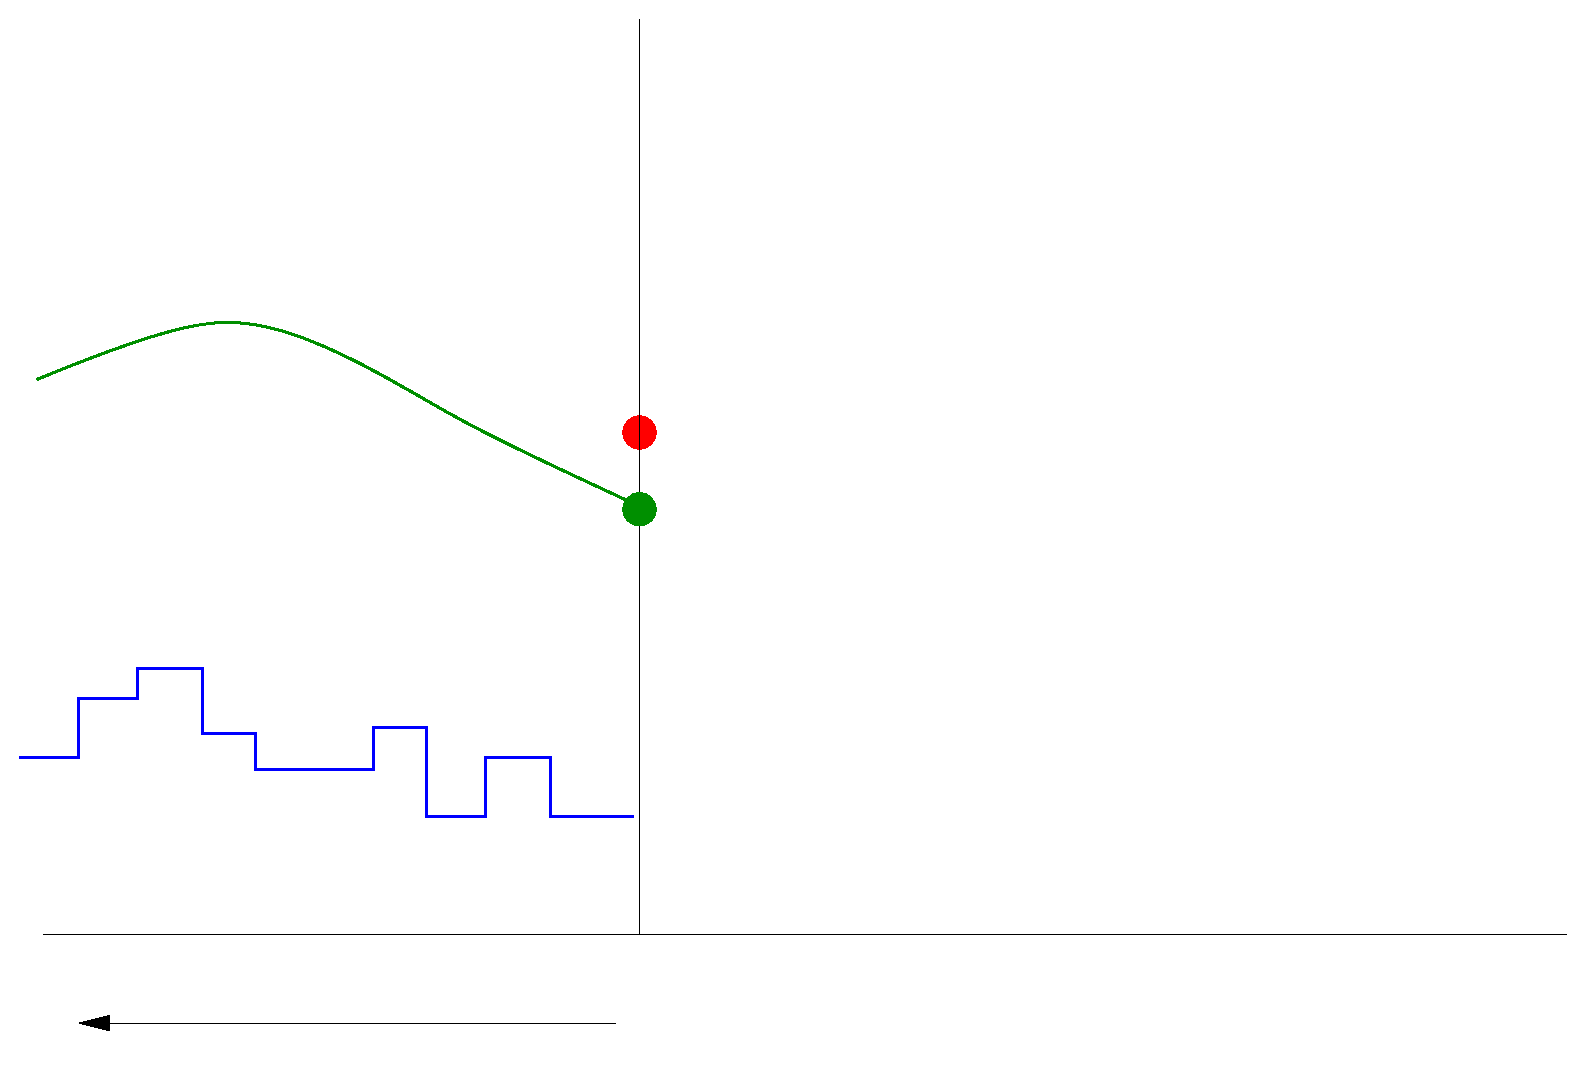
\includegraphics{mpc}%
\end{picture}%
\setlength{\unitlength}{4144sp}%
%
\begingroup\makeatletter\ifx\SetFigFont\undefined%
\gdef\SetFigFont#1#2#3#4#5{%
  \reset@font\fontsize{#1}{#2pt}%
  \fontfamily{#3}\fontseries{#4}\fontshape{#5}%
  \selectfont}%
\fi\endgroup%
\begin{picture}(11824,7992)(1329,-8266)
\put(1531,-3616){\makebox(0,0)[lb]{\smash{{\SetFigFont{25}{30.0}{\rmdefault}{\mddefault}{\updefault}{\color[rgb]{0,0,0}State}%
}}}}
\put(5986,-7531){\makebox(0,0)[lb]{\smash{{\SetFigFont{14}{16.8}{\rmdefault}{\mddefault}{\updefault}{\color[rgb]{0,0,0}$k$}%
}}}}
\put(2206,-8251){\makebox(0,0)[lb]{\smash{{\SetFigFont{14}{16.8}{\rmdefault}{\mddefault}{\updefault}{\color[rgb]{0,0,0}Past}%
}}}}
\put(1441,-6271){\makebox(0,0)[lb]{\smash{{\SetFigFont{14}{16.8}{\rmdefault}{\mddefault}{\updefault}{\color[rgb]{0,0,0}$u$}%
}}}}
\put(6301,-3541){\makebox(0,0)[lb]{\smash{{\SetFigFont{14}{16.8}{\rmdefault}{\mddefault}{\updefault}{\color[rgb]{0,0,0}$\hat{x}$}%
}}}}
\put(1441,-6631){\makebox(0,0)[lb]{\smash{{\SetFigFont{25}{30.0}{\rmdefault}{\mddefault}{\updefault}{\color[rgb]{0,0,0}Input}%
}}}}
\put(6301,-3256){\makebox(0,0)[lb]{\smash{{\SetFigFont{25}{30.0}{\rmdefault}{\mddefault}{\updefault}{\color[rgb]{0,0,0}Estimated state}%
}}}}
\put(9766,-3436){\makebox(0,0)[lb]{\smash{{\SetFigFont{17}{20.4}{\rmdefault}{\mddefault}{\updefault}{\color[rgb]{0,0,0}{\color{blue}{$x(k+1) = Ax(k) + Bu(k)$}}}%
}}}}
\put(9721,-2986){\makebox(0,0)[lb]{\smash{{\SetFigFont{29}{34.8}{\rmdefault}{\mddefault}{\updefault}{\color{red}{Process Model}}}}}}
\put(1531,-3301){\makebox(0,0)[lb]{\smash{{\SetFigFont{14}{16.8}{\rmdefault}{\mddefault}{\updefault}{\color[rgb]{0,0,0}$x$}%
}}}}
\end{picture}%
}}
  \end{figure}
\onslide<2|handout:0>
\begin{figure}
    \centering
    \huge{\resizebox{1\textwidth}{!}{\begin{picture}(0,0)%
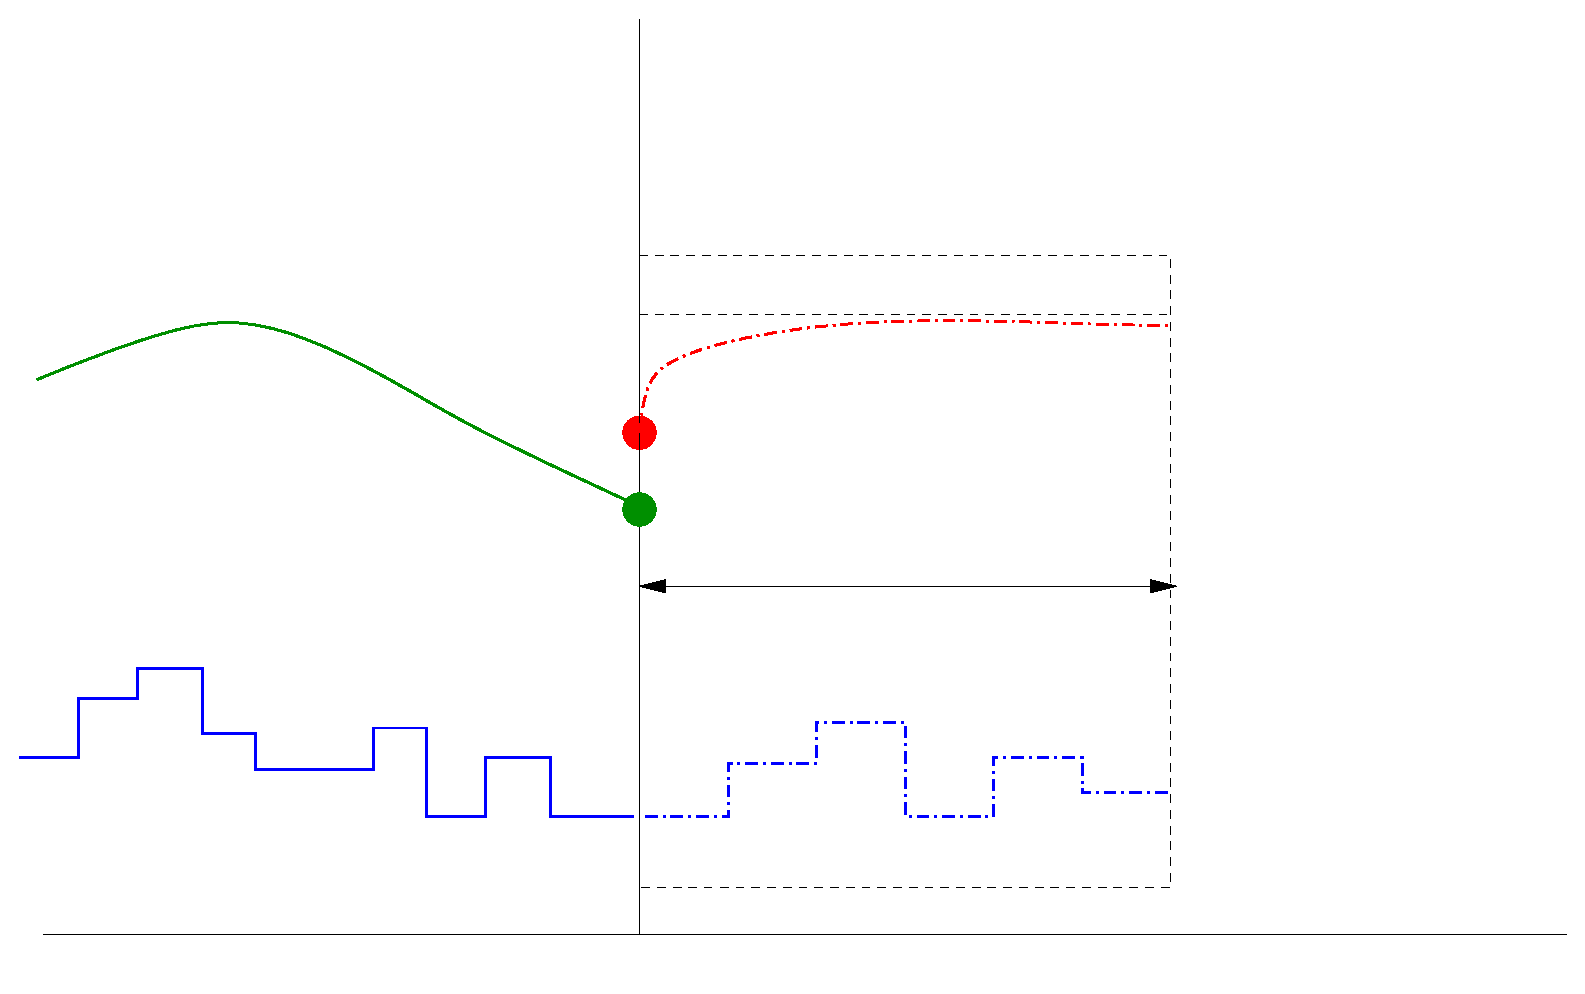
\includegraphics{mpc1}%
\end{picture}%
\setlength{\unitlength}{4144sp}%
%
\begingroup\makeatletter\ifx\SetFigFont\undefined%
\gdef\SetFigFont#1#2#3#4#5{%
  \reset@font\fontsize{#1}{#2pt}%
  \fontfamily{#3}\fontseries{#4}\fontshape{#5}%
  \selectfont}%
\fi\endgroup%
\begin{picture}(11824,7312)(1329,-7586)
\put(10531,-3436){\makebox(0,0)[lb]{\smash{{\SetFigFont{20}{24.0}{\rmdefault}{\mddefault}{\updefault}{\color[rgb]{0,0,0}{\color{blue}{Optimization}}}%
}}}}
\put(5986,-7531){\makebox(0,0)[lb]{\smash{{\SetFigFont{14}{16.8}{\rmdefault}{\mddefault}{\updefault}{\color[rgb]{0,0,0}$k$}%
}}}}
\put(1441,-6271){\makebox(0,0)[lb]{\smash{{\SetFigFont{14}{16.8}{\rmdefault}{\mddefault}{\updefault}{\color[rgb]{0,0,0}$u$}%
}}}}
\put(9901,-7486){\makebox(0,0)[lb]{\smash{{\SetFigFont{14}{16.8}{\rmdefault}{\mddefault}{\updefault}{\color[rgb]{0,0,0}$k+N$}%
}}}}
\put(1531,-3301){\makebox(0,0)[lb]{\smash{{\SetFigFont{14}{16.8}{\rmdefault}{\mddefault}{\updefault}{\color[rgb]{0,0,0}$x$}%
}}}}
\put(1531,-3616){\makebox(0,0)[lb]{\smash{{\SetFigFont{25}{30.0}{\rmdefault}{\mddefault}{\updefault}{\color[rgb]{0,0,0}State}%
}}}}
\put(1441,-6631){\makebox(0,0)[lb]{\smash{{\SetFigFont{25}{30.0}{\rmdefault}{\mddefault}{\updefault}{\color[rgb]{0,0,0}Input}%
}}}}
\put(9676,-2491){\makebox(0,0)[lb]{\smash{{\SetFigFont{14}{16.8}{\rmdefault}{\mddefault}{\updefault}{\color[rgb]{0,0,0}Set point}%
}}}}
\put(6796,-5461){\makebox(0,0)[lb]{\smash{{\SetFigFont{14}{16.8}{\rmdefault}{\mddefault}{\updefault}{\color[rgb]{0,0,0}Optimized future input trajectory}%
}}}}
\put(6796,-2986){\makebox(0,0)[lb]{\smash{{\SetFigFont{14}{16.8}{\rmdefault}{\mddefault}{\updefault}{\color[rgb]{0,0,0}Predicted future output trajectory}%
}}}}
\put(6796,-4516){\makebox(0,0)[lb]{\smash{{\SetFigFont{14}{16.8}{\rmdefault}{\mddefault}{\updefault}{\color[rgb]{0,0,0}Control Horizon $N$}%
}}}}
\put(10576,-3886){\makebox(0,0)[lb]{\smash{{\SetFigFont{17}{20.4}{\rmdefault}{\mddefault}{\updefault}{\color[rgb]{0,0,1}$\min_{\mathbf{u}}{\sum_{i=k}^{i=k+N-1}\ell(x(i),u(i))}$}%
}}}}
\put(10576,-4381){\makebox(0,0)[lb]{\smash{{\SetFigFont{17}{20.4}{\rmdefault}{\mddefault}{\updefault}{\color[rgb]{0,0,1}$\text{s.t.~}x^+ = Ax+Bu;$}%
}}}}
\put(10576,-4786){\makebox(0,0)[lb]{\smash{{\SetFigFont{17}{20.4}{\rmdefault}{\mddefault}{\updefault}{\color[rgb]{0,0,1}$x \in \mathbb{X}$}%
}}}}
\put(10576,-5191){\makebox(0,0)[lb]{\smash{{\SetFigFont{17}{20.4}{\rmdefault}{\mddefault}{\updefault}{\color[rgb]{0,0,1}$u \in \mathbb{U}$}%
}}}}
\end{picture}%
}}
  \end{figure}
\onslide<3|handout:1>
\begin{figure}
    \centering
    \huge{\resizebox{1\textwidth}{!}{\begin{picture}(0,0)%
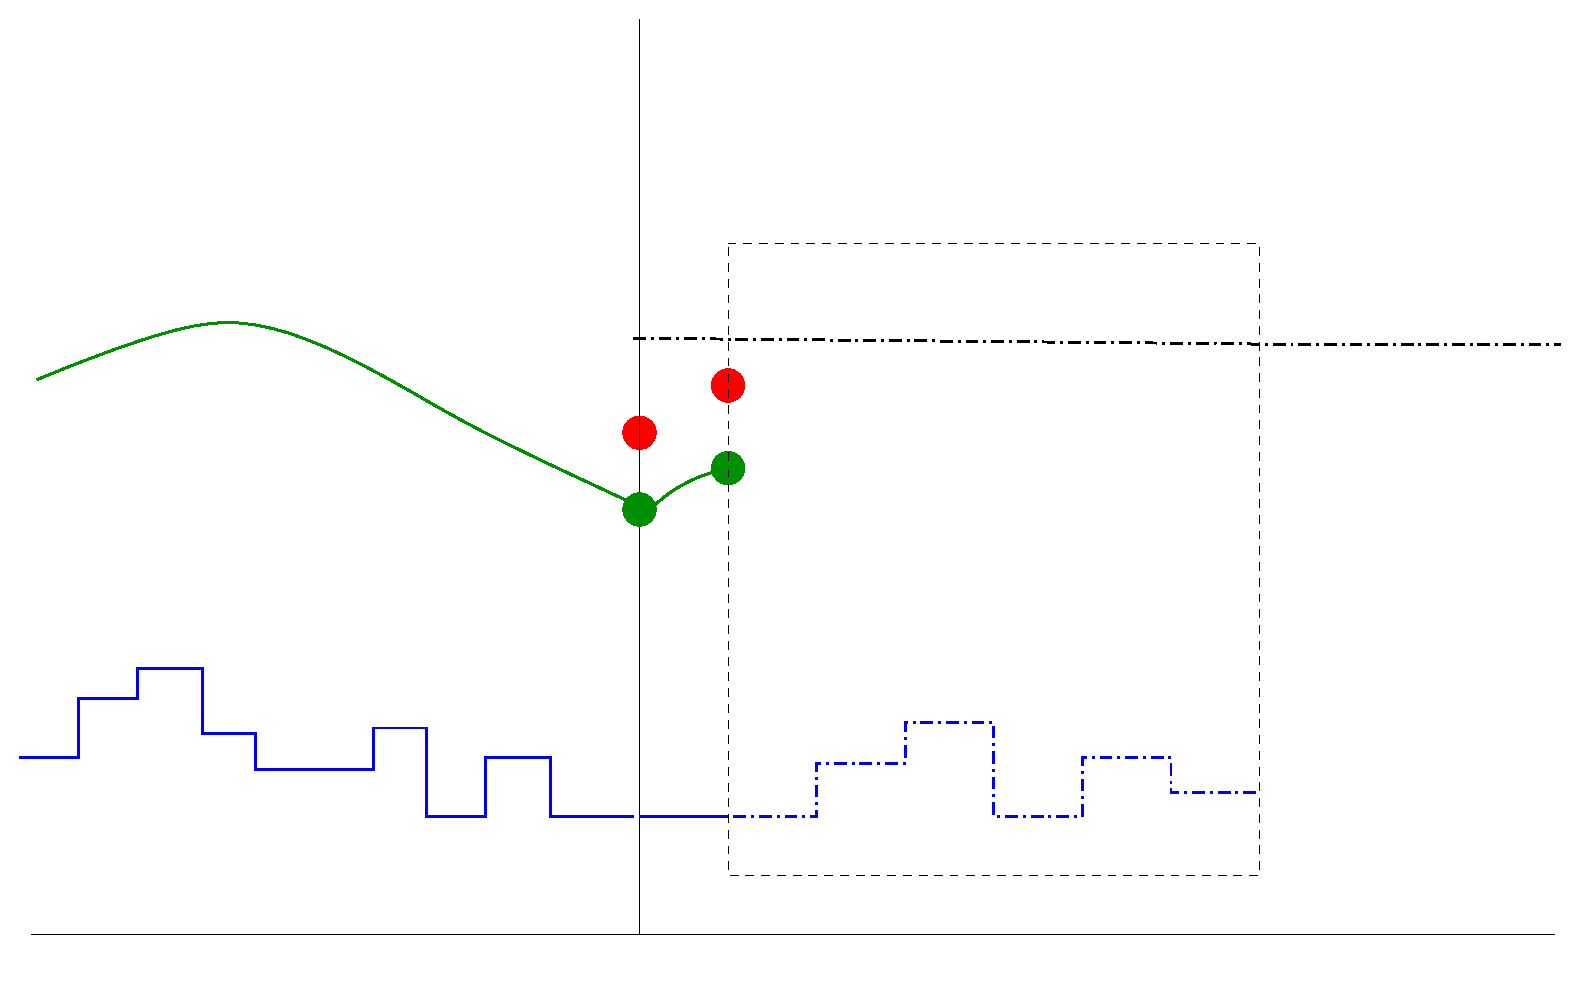
\includegraphics{mpc2}%
\end{picture}%
\setlength{\unitlength}{4144sp}%
%
\begingroup\makeatletter\ifx\SetFigFont\undefined%
\gdef\SetFigFont#1#2#3#4#5{%
  \reset@font\fontsize{#1}{#2pt}%
  \fontfamily{#3}\fontseries{#4}\fontshape{#5}%
  \selectfont}%
\fi\endgroup%
\begin{picture}(11789,7312)(1329,-7586)
\put(7426,-3966){\makebox(0,0)[lb]{\smash{{\SetFigFont{20}{24.0}{\rmdefault}{\mddefault}{\updefault}{\color[rgb]{0,0,0}{\color{blue}{Repeat procedure at $k+1$}}}%
}}}}
\put(5986,-7531){\makebox(0,0)[lb]{\smash{{\SetFigFont{14}{16.8}{\rmdefault}{\mddefault}{\updefault}{\color[rgb]{0,0,0}$k$}%
}}}}
\put(1441,-6271){\makebox(0,0)[lb]{\smash{{\SetFigFont{14}{16.8}{\rmdefault}{\mddefault}{\updefault}{\color[rgb]{0,0,0}$u$}%
}}}}
\put(1441,-6631){\makebox(0,0)[lb]{\smash{{\SetFigFont{25}{30.0}{\rmdefault}{\mddefault}{\updefault}{\color[rgb]{0,0,0}Input}%
}}}}
\put(1531,-3301){\makebox(0,0)[lb]{\smash{{\SetFigFont{14}{16.8}{\rmdefault}{\mddefault}{\updefault}{\color[rgb]{0,0,0}$x$}%
}}}}
\put(1531,-3616){\makebox(0,0)[lb]{\smash{{\SetFigFont{25}{30.0}{\rmdefault}{\mddefault}{\updefault}{\color[rgb]{0,0,0}State}%
}}}}
\put(6706,-7531){\makebox(0,0)[lb]{\smash{{\SetFigFont{14}{16.8}{\rmdefault}{\mddefault}{\updefault}{\color[rgb]{0,0,0}$k+1$}%
}}}}
\put(10666,-7486){\makebox(0,0)[lb]{\smash{{\SetFigFont{14}{16.8}{\rmdefault}{\mddefault}{\updefault}{\color[rgb]{0,0,0}$k+N+1$}%
}}}}
\put(7426,-3571){\makebox(0,0)[lb]{\smash{{\SetFigFont{20}{24.0}{\rmdefault}{\mddefault}{\updefault}{\color[rgb]{0,0,0}{\color{red}{Implement first move from the optimal sequence}}}%
}}}}
\end{picture}%
}}
  \end{figure}
\end{overprint}
\end{frame}

{\FooterCite{\citet{beamon:1998,angerhofer:angelides:2000,shah:2005}}
\begin{frame}{Supply chain modeling}
 \begin{figure}
  \centering
  \huge{\resizebox{0.7\textwidth}{!}{\begin{picture}(0,0)%
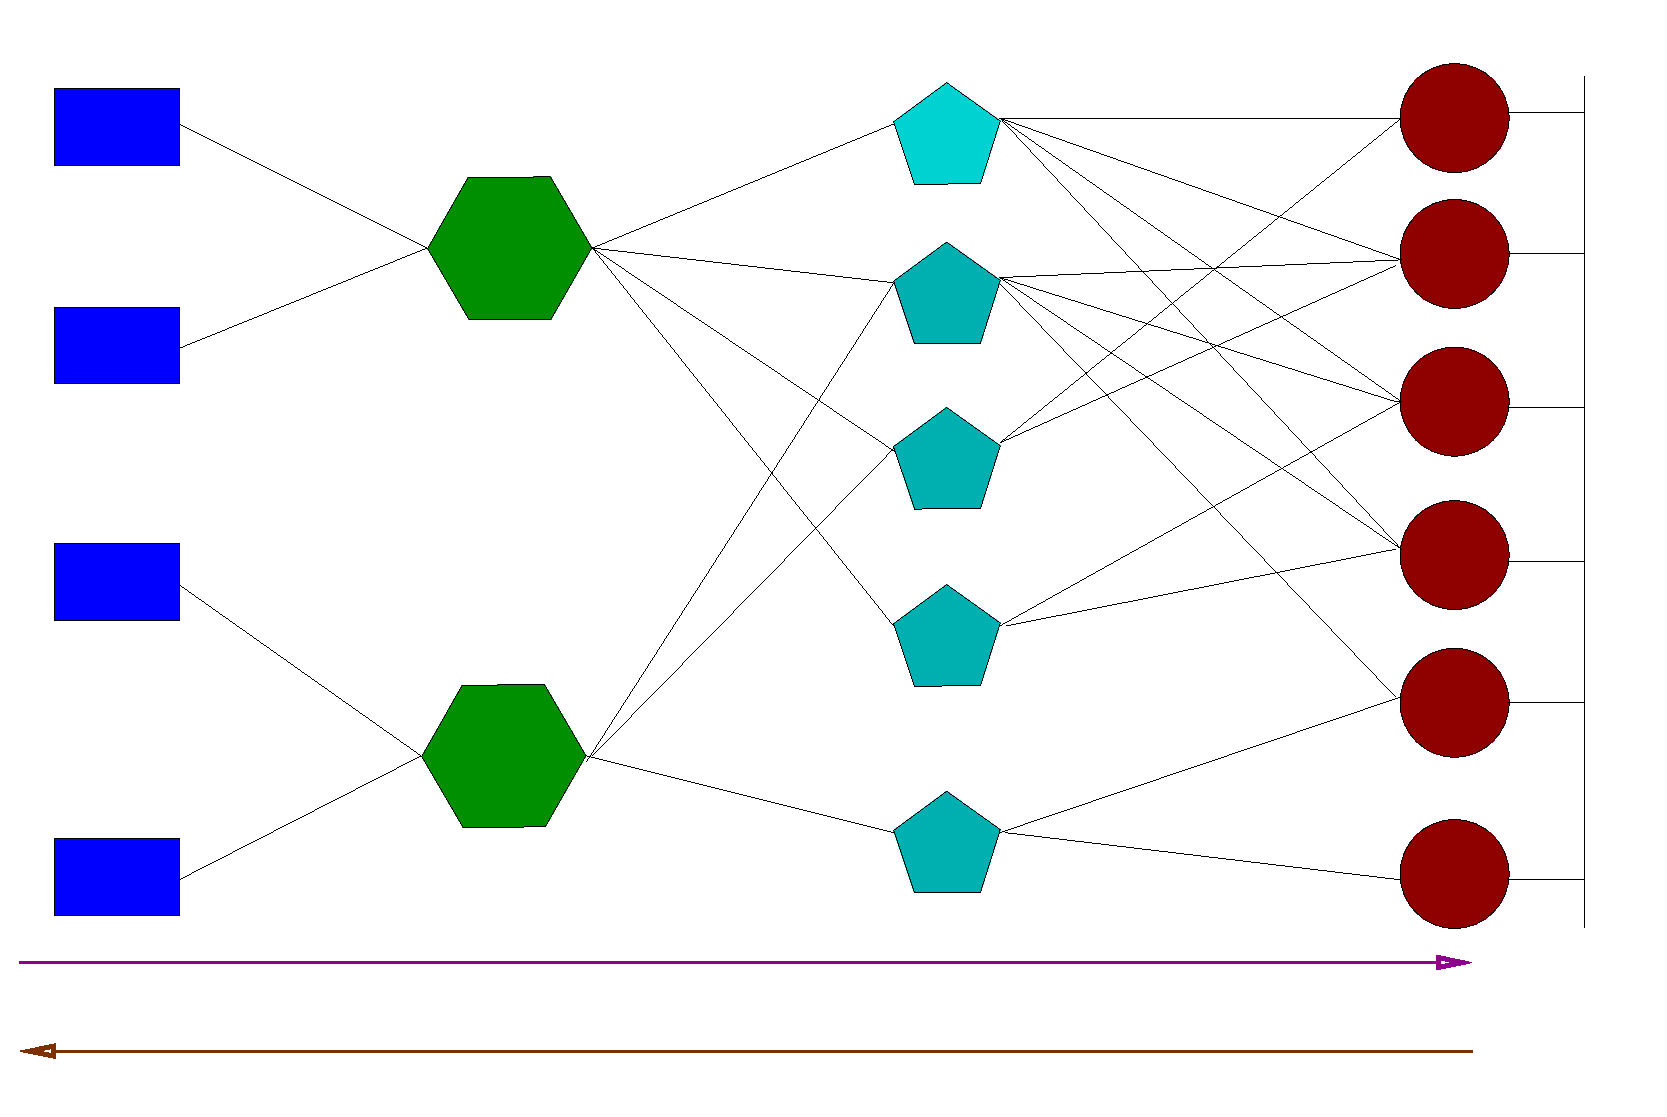
\includegraphics{sc/nodes1_color}%
\end{picture}%
\setlength{\unitlength}{4144sp}%
%
\begingroup\makeatletter\ifx\SetFigFont\undefined%
\gdef\SetFigFont#1#2#3#4#5{%
  \reset@font\fontsize{#1}{#2pt}%
  \fontfamily{#3}\fontseries{#4}\fontshape{#5}%
  \selectfont}%
\fi\endgroup%
\begin{picture}(12502,8244)(744,-8131)
\put(13231,-2626){\rotatebox{90.0}{\makebox(0,0)[rb]{\smash{{\SetFigFont{14}{16.8}{\rmdefault}{\mddefault}{\updefault}{\color[rgb]{0,0,0}CUSTOMERS}%
}}}}}
\put(9091,-7351){\makebox(0,0)[lb]{\smash{{\SetFigFont{17}{20.4}{\familydefault}{\mddefault}{\updefault}{\color[rgb]{.56,0,.56}Product Flow}%
}}}}
\put(946,-106){\makebox(0,0)[lb]{\smash{{\SetFigFont{17}{20.4}{\familydefault}{\mddefault}{\updefault}{\color[rgb]{0,0,1}Suppliers}%
}}}}
\put(7156,-106){\makebox(0,0)[lb]{\smash{{\SetFigFont{17}{20.4}{\familydefault}{\mddefault}{\updefault}{\color[rgb]{0,.69,.69}Distibution}%
}}}}
\put(7381,-331){\makebox(0,0)[lb]{\smash{{\SetFigFont{17}{20.4}{\familydefault}{\mddefault}{\updefault}{\color[rgb]{0,.69,.69}Centers}%
}}}}
\put(3826,-151){\makebox(0,0)[lb]{\smash{{\SetFigFont{17}{20.4}{\familydefault}{\mddefault}{\updefault}{\color[rgb]{0,.56,0}Production }%
}}}}
\put(4051,-511){\makebox(0,0)[lb]{\smash{{\SetFigFont{17}{20.4}{\familydefault}{\mddefault}{\updefault}{\color[rgb]{0,.56,0}Facility}%
}}}}
\put(11161,-106){\makebox(0,0)[lb]{\smash{{\SetFigFont{17}{20.4}{\familydefault}{\mddefault}{\updefault}{\color[rgb]{.56,0,0}Retailers}%
}}}}
\put(1396,-8116){\makebox(0,0)[lb]{\smash{{\SetFigFont{17}{20.4}{\familydefault}{\mddefault}{\updefault}{\color[rgb]{.5,.17,0}Information Flow}%
}}}}
\end{picture}%
}}
 \end{figure}
 \begin{itemize}
  \item Each unit is a node.
  \item Every connection indicates two types of flows between the
     nodes. 
 \end{itemize}
\end{frame}
}

\begin{frame}{Modeling a node}
 \begin{figure}
  \centering      
  \huge{\resizebox{0.65\textwidth}{!}{\begin{picture}(0,0)%
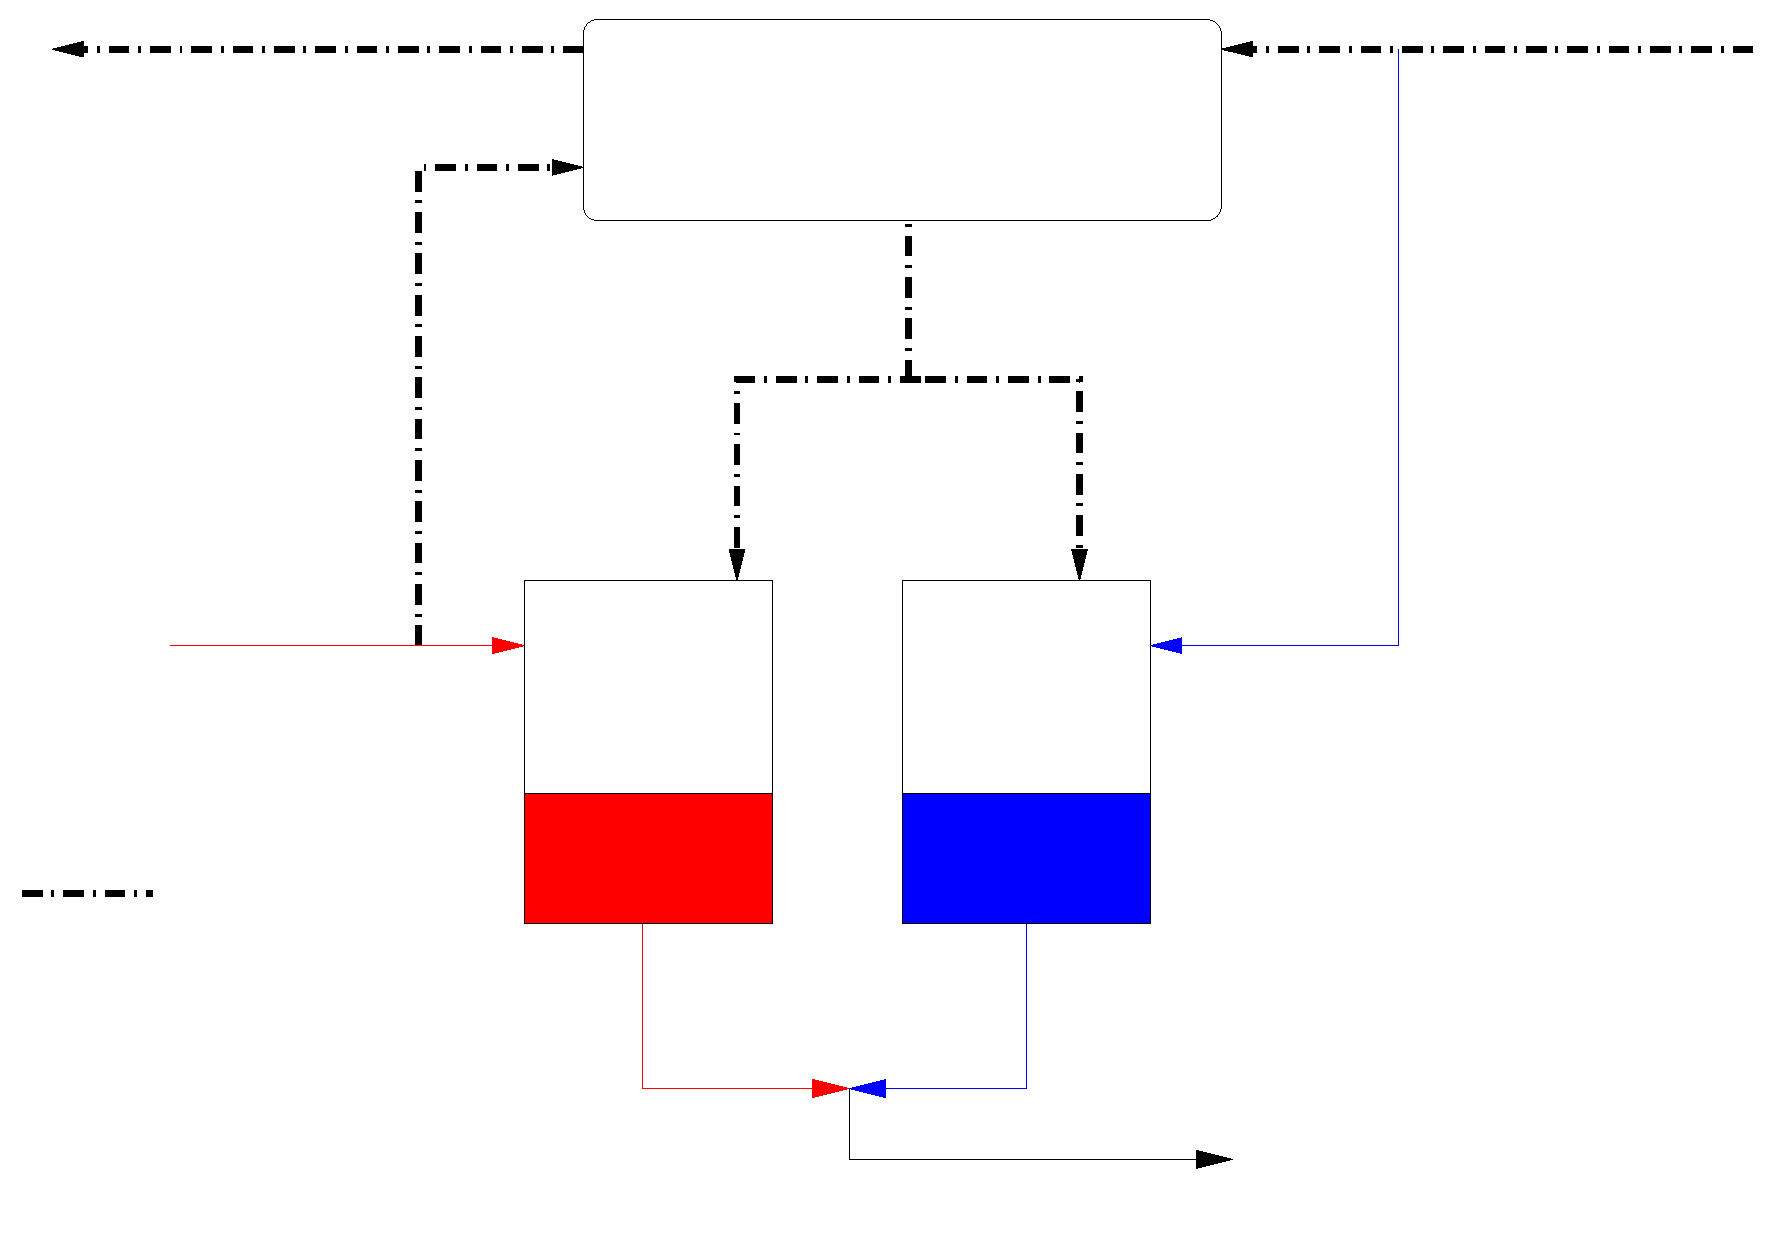
\includegraphics{model}%
\end{picture}%
\setlength{\unitlength}{4144sp}%
%
\begingroup\makeatletter\ifx\SetFigFont\undefined%
\gdef\SetFigFont#1#2#3#4#5{%
  \reset@font\fontsize{#1}{#2pt}%
  \fontfamily{#3}\fontseries{#4}\fontshape{#5}%
  \selectfont}%
\fi\endgroup%
\begin{picture}(13539,9207)(407,-8671)
\put(6841,-646){\makebox(0,0)[b]{\smash{{\SetFigFont{20}{24.0}{\rmdefault}{\mddefault}{\updefault}{\color[rgb]{0,0,0}(policy implementer/optimizer)}%
}}}}
\put(10486,-5191){\makebox(0,0)[lb]{\smash{{\SetFigFont{20}{24.0}{\rmdefault}{\mddefault}{\updefault}{\color[rgb]{0,0,0}Information sharing}%
}}}}
\put(4321,-4876){\makebox(0,0)[lb]{\smash{{\SetFigFont{20}{24.0}{\rmdefault}{\mddefault}{\updefault}{\color[rgb]{0,0,0}Inventory}%
}}}}
\put(7471,-5011){\makebox(0,0)[lb]{\smash{{\SetFigFont{20}{24.0}{\rmdefault}{\mddefault}{\updefault}{\color[rgb]{0,0,0}Orders}%
}}}}
\put(7471,-4696){\makebox(0,0)[lb]{\smash{{\SetFigFont{20}{24.0}{\rmdefault}{\mddefault}{\updefault}{\color[rgb]{0,0,0}Back-}%
}}}}
\put(721,-61){\makebox(0,0)[lb]{\smash{{\SetFigFont{20}{24.0}{\rmdefault}{\mddefault}{\updefault}{\color[rgb]{0,0,0}Orders}%
}}}}
\put(721,-361){\makebox(0,0)[lb]{\smash{{\SetFigFont{20}{24.0}{\rmdefault}{\mddefault}{\updefault}{\color[rgb]{0,0,0}(placed to }%
}}}}
\put(721,-661){\makebox(0,0)[lb]{\smash{{\SetFigFont{20}{24.0}{\rmdefault}{\mddefault}{\updefault}{\color[rgb]{0,0,0}upstream nodes)}%
}}}}
\put(11116,-61){\makebox(0,0)[lb]{\smash{{\SetFigFont{20}{24.0}{\rmdefault}{\mddefault}{\updefault}{\color[rgb]{0,0,0}Orders}%
}}}}
\put(11116,-376){\makebox(0,0)[lb]{\smash{{\SetFigFont{20}{24.0}{\rmdefault}{\mddefault}{\updefault}{\color[rgb]{0,0,0}(placed by}%
}}}}
\put(11116,-646){\makebox(0,0)[lb]{\smash{{\SetFigFont{20}{24.0}{\rmdefault}{\mddefault}{\updefault}{\color[rgb]{0,0,0}downstream nodes)}%
}}}}
\put(9676,-8566){\makebox(0,0)[lb]{\smash{{\SetFigFont{20}{24.0}{\rmdefault}{\mddefault}{\updefault}{\color[rgb]{0,0,0}(Demands satisfied)}%
}}}}
\put(9631,-8206){\makebox(0,0)[lb]{\smash{{\SetFigFont{20}{24.0}{\rmdefault}{\mddefault}{\updefault}{\color[rgb]{0,0,0}(to downstream nodes)}%
}}}}
\put(9631,-7846){\makebox(0,0)[lb]{\smash{{\SetFigFont{20}{24.0}{\rmdefault}{\mddefault}{\updefault}{\color[rgb]{0,0,0}Shipments }%
}}}}
\put(676,-4651){\makebox(0,0)[lb]{\smash{{\SetFigFont{20}{24.0}{\rmdefault}{\mddefault}{\updefault}{\color[rgb]{0,0,0}Shipments}%
}}}}
\put(676,-4951){\makebox(0,0)[lb]{\smash{{\SetFigFont{20}{24.0}{\rmdefault}{\mddefault}{\updefault}{\color[rgb]{0,0,0}(from upstream nodes)}%
}}}}
\put(6841,-196){\makebox(0,0)[b]{\smash{{\SetFigFont{20}{24.0}{\rmdefault}{\mddefault}{\updefault}{\color[rgb]{0,0,0}Decision Maker}%
}}}}
\end{picture}%
}}
 \end{figure}
 \begin{itemize}
  \item States: inventory, back-orders
  \item Inputs: shipments, orders
  \item Disturbances: inputs of other nodes, customer demand
  \item \alert{Interconnected system of integrators}
 \end{itemize} 
\end{frame}

\begin{frame}
\frametitle{Assembling the (centralized) supply chain model}
\begin{itemize}
\item State $x$: Inventories and back-orders in all nodes
\item Input $u$: Shipment and orders out of every node
\item Disturbance $d$: Customer demands
\item Model $x(k+1) = Ax(k) + Bu(k) + B_dd(k)$
\item State constraints $x^{lb} \leq x \leq x^{ub}$, e.g.  safety
  inventory, capacity limits etc.
\item Input constraints $u^{lb} \leq u \leq u^{ub}$, e.g. transportation constraints, production constraints etc.
\item Objective function
 \begin{itemize}
   \item Profit = Revenue-Operating costs
   \item Tracking targets $x_t$,$u_t$, like  inventory targets etc.
\end{itemize}
\item \alert{ MIMO control problem with input and state constraints.}
\end{itemize}
\end{frame}
{\FooterCite{\citet{shah:pantelides:sargent:1993}}
\begin{frame}[t]{Modeling the manufacturing facility}
\begin{columns}[T]
\column{0.6\textwidth}
\begin{itemize}
\item \alert{State task network}
\begin{itemize}
 \item Processing units $j \in \mathbf{J}$
 \item Processing tasks $i \in \mathbf{I}$ (duration: $\tau_i$,
   batchsize: $\beta_i$)
 \item Materials $k \in \mathbf{K}$ (storage capacity $\sigma_k$)
\end{itemize}
\item \alert{Discrete-time representation}
  \begin{itemize}
    \item Horizon $\eta$, partitioned into $T$ time periods
   \end{itemize}
\item \alert{Decision variables}
  \begin{itemize}
    \item $W_{i,t} \in \set{0,1} = 1$ if task $i$ starts at time point
      $t$
    \item $S_{k,t} \in [0,\sigma_k]$: inventory level of material $k$ at
      time $t$
\end{itemize}
\item \alert{Mixed-integer programming model}
\begin{itemize}
 \item Resource constraint
 \item Material balance
\end{itemize}
\end{itemize}
\column{0.4\textwidth}
\begin{figure}
  \centering
  \resizebox{1\columnwidth}{!}{\begin{picture}(0,0)%
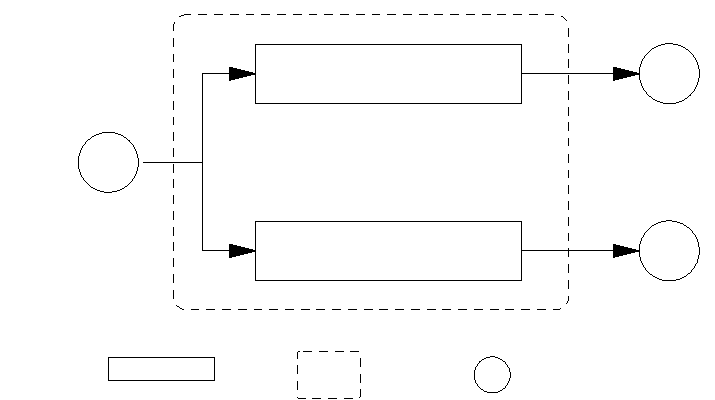
\includegraphics{scheduling/ABexample}%
\end{picture}%
\setlength{\unitlength}{4144sp}%
%
\begingroup\makeatletter\ifx\SetFigFont\undefined%
\gdef\SetFigFont#1#2#3#4#5{%
  \reset@font\fontsize{#1}{#2pt}%
  \fontfamily{#3}\fontseries{#4}\fontshape{#5}%
  \selectfont}%
\fi\endgroup%
\begin{picture}(5430,3041)(76,-3447)
\put( 91,-1726){\makebox(0,0)[lb]{\smash{{\SetFigFont{17}{20.4}{\rmdefault}{\mddefault}{\updefault}{\color[rgb]{0,.56,0}RM}%
}}}}
\put(3061,-3301){\makebox(0,0)[lb]{\smash{{\SetFigFont{17}{20.4}{\rmdefault}{\mddefault}{\updefault}{\color[rgb]{0,0,0}Unit}%
}}}}
\put(4141,-3301){\makebox(0,0)[lb]{\smash{{\SetFigFont{17}{20.4}{\rmdefault}{\mddefault}{\updefault}{\color[rgb]{0,0,0}Material}%
}}}}
\put(1801,-3301){\makebox(0,0)[lb]{\smash{{\SetFigFont{17}{20.4}{\rmdefault}{\mddefault}{\updefault}{\color[rgb]{0,0,0}Task}%
}}}}
\put(2971,-1051){\makebox(0,0)[lb]{\smash{{\SetFigFont{17}{20.4}{\rmdefault}{\mddefault}{\updefault}{\color[rgb]{0,0,0}TA}%
}}}}
\put(2971,-2401){\makebox(0,0)[lb]{\smash{{\SetFigFont{17}{20.4}{\rmdefault}{\mddefault}{\updefault}{\color[rgb]{0,0,0}TB}%
}}}}
\put(1126,-556){\makebox(0,0)[lb]{\smash{{\SetFigFont{17}{20.4}{\rmdefault}{\mddefault}{\updefault}{\color[rgb]{0,0,0}U}%
}}}}
\put(1801,-1996){\makebox(0,0)[lb]{\smash{{\SetFigFont{17}{20.4}{\rmdefault}{\mddefault}{\updefault}{\color[rgb]{0,0,0}$\tau_{TB}=2$hr, $\beta_{TB}=6$ton}%
}}}}
\put(1801,-1411){\makebox(0,0)[lb]{\smash{{\SetFigFont{17}{20.4}{\rmdefault}{\mddefault}{\updefault}{\color[rgb]{0,0,0}$\tau_{TA}=3$hr, $\beta_{TA}=4$ton }%
}}}}
\put(5491,-2401){\makebox(0,0)[lb]{\smash{{\SetFigFont{17}{20.4}{\rmdefault}{\mddefault}{\updefault}{\color[rgb]{1,0,0}$B$}%
}}}}
\put(5491,-1006){\makebox(0,0)[lb]{\smash{{\SetFigFont{17}{20.4}{\rmdefault}{\mddefault}{\updefault}{\color[rgb]{0,0,1}$A$}%
}}}}
\end{picture}%
}
  %\caption{Simple scheduling problem}
  %\label{fig:scheduling:ABexample}
\end{figure}

\begin{figure}[h]
  \centering
  \resizebox{1\columnwidth}{!}{\begin{picture}(0,0)%
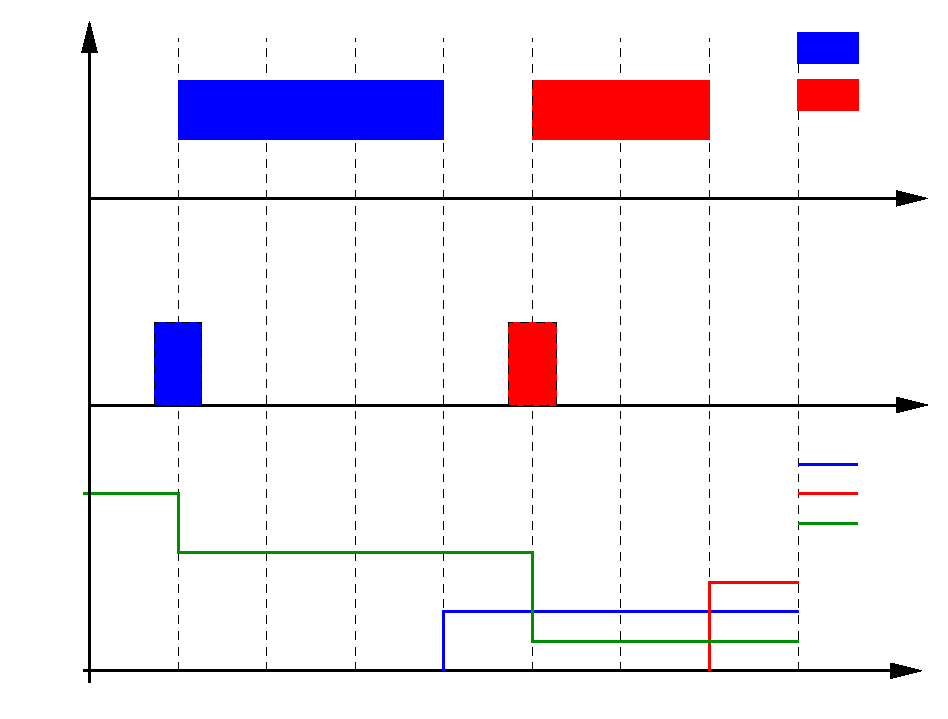
\includegraphics{ABgantt}%
\end{picture}%
\setlength{\unitlength}{4144sp}%
%
\begingroup\makeatletter\ifx\SetFigFont\undefined%
\gdef\SetFigFont#1#2#3#4#5{%
  \reset@font\fontsize{#1}{#2pt}%
  \fontfamily{#3}\fontseries{#4}\fontshape{#5}%
  \selectfont}%
\fi\endgroup%
\begin{picture}(6967,5212)(1471,-5476)
\put(2926,-2536){\makebox(0,0)[lb]{\smash{{\SetFigFont{17}{20.4}{\rmdefault}{\mddefault}{\updefault}{\color[rgb]{0,0,0}$W_{TA,1}=1$}%
}}}}
\put(2701,-421){\makebox(0,0)[lb]{\smash{{\SetFigFont{17}{20.4}{\rmdefault}{\mddefault}{\updefault}{\color[rgb]{0,0,0}Gantt Chart}%
}}}}
\put(2701,-3571){\makebox(0,0)[lb]{\smash{{\SetFigFont{17}{20.4}{\rmdefault}{\mddefault}{\updefault}{\color[rgb]{0,0,0}Inventory profile}%
}}}}
\put(8101,-556){\makebox(0,0)[lb]{\smash{{\SetFigFont{17}{20.4}{\rmdefault}{\mddefault}{\updefault}{\color[rgb]{0,0,0}TA}%
}}}}
\put(8101,-916){\makebox(0,0)[lb]{\smash{{\SetFigFont{17}{20.4}{\rmdefault}{\mddefault}{\updefault}{\color[rgb]{0,0,0}TB}%
}}}}
\put(7966,-3706){\makebox(0,0)[lb]{\smash{{\SetFigFont{17}{20.4}{\rmdefault}{\mddefault}{\updefault}{\color[rgb]{0,0,0}$S_{A,t}$}%
}}}}
\put(7966,-3931){\makebox(0,0)[lb]{\smash{{\SetFigFont{17}{20.4}{\rmdefault}{\mddefault}{\updefault}{\color[rgb]{0,0,0}$S_{B,t}$}%
}}}}
\put(7966,-4156){\makebox(0,0)[lb]{\smash{{\SetFigFont{17}{20.4}{\rmdefault}{\mddefault}{\updefault}{\color[rgb]{0,0,0}$S_{RM,t}$}%
}}}}
\put(1486,-2356){\makebox(0,0)[lb]{\smash{{\SetFigFont{17}{20.4}{\rmdefault}{\mddefault}{\updefault}{\color[rgb]{0,0,0}$W_{i,t}$}%
}}}}
\put(7831,-5461){\makebox(0,0)[lb]{\smash{{\SetFigFont{17}{20.4}{\rmdefault}{\mddefault}{\updefault}{\color[rgb]{0,0,0}Time}%
}}}}
\put(3376,-5416){\makebox(0,0)[lb]{\smash{{\SetFigFont{17}{20.4}{\rmdefault}{\mddefault}{\updefault}{\color[rgb]{0,0,0}2}%
}}}}
\put(4726,-5416){\makebox(0,0)[lb]{\smash{{\SetFigFont{17}{20.4}{\rmdefault}{\mddefault}{\updefault}{\color[rgb]{0,0,0}4}%
}}}}
\put(6076,-5416){\makebox(0,0)[lb]{\smash{{\SetFigFont{17}{20.4}{\rmdefault}{\mddefault}{\updefault}{\color[rgb]{0,0,0}6}%
}}}}
\put(7426,-5416){\makebox(0,0)[lb]{\smash{{\SetFigFont{17}{20.4}{\rmdefault}{\mddefault}{\updefault}{\color[rgb]{0,0,0}8}%
}}}}
\put(5626,-2536){\makebox(0,0)[lb]{\smash{{\SetFigFont{17}{20.4}{\rmdefault}{\mddefault}{\updefault}{\color[rgb]{0,0,0}$W_{TB,5}=1$}%
}}}}
\end{picture}%
}
  %\caption{Scheduling solution}
  %\label{fig:scheduling:ABgantt}
\end{figure}
\end{columns}
\end{frame}
}


\begin{frame}{Outline-I}
\begin{itemize}
 \item Detailed optimization model + rolling horizon guarantees \ldots \\   
 \centerline{\alert{no reasonable closed-loop properties!}}  
 \item Examples:
 \begin{enumerate}
  \item Supply chain minimizing costs does not meet customer demands  
  \item Manufacturing facility cannot find feasible schedules  
 \end{enumerate} 
  \item Rolling horizon + MPC design guarantees
    \ldots \\  
  \centerline{\alert{favorable closed-loop properties like stability, convergence.}}   
  \item Contributions:
  \begin{enumerate}
   \item {\color{blue}{Stability and convergence guarantees for supply
         chain using Economic MPC}} 
   \item {\color{blue}{Recursive feasibility and rescheduling
         techniques for iterative scheduling}}
  \end{enumerate}
 \end{itemize}
\end{frame}

\begin{frame}{Outline-II}
\begin{itemize}
\item Distributed nature of supply chain decision making \\
   
 \centerline{\alert{ How to coordinate multiple decision makers?}}  
\item Sharing information does not imply better
  solutions\footnote{minimize overall system cost}   

\item \alert{Distributed} MPC enables use of many interacting decision
  makers to improve overall system performance\footnotemark[\value{footnote}]  

\item Contributions:
 \begin{enumerate}
   \item {\color{blue}{Stability \& convergence guarantees extended to cover supply
     chain models}}  
   \item {\color{blue} {Robust cooperative MPC to design controllers
       that are robust to demand fluctuations}}
 \end{enumerate}
\end{itemize}
\end{frame}

{\NoHeaderFooter
\begin{frame}{Outline-I}
\addtocounter{framenumber}{-1}
\begin{itemize}
 \item {{Detailed optimization model + rolling horizon guarantees \ldots \\ 
 \centerline{{no reasonable closed-loop properties!}}}}
 \item Examples:
 \begin{enumerate}
  \item \alert{Supply chain minimizing costs does not meet customer demands }
  {\color{gray}{
  \item Manufacturing facility cannot find feasible schedules }}
 \end{enumerate} 
% \end{itemize}
%\end{exampleblock} 
%\begin{block}{}
% \begin{itemize}
  \item Rolling horizon + MPC design guarantees
    \ldots \\ 
  \centerline{{favorable closed-loop properties like stability, convergence.}} 
  \item Contributions:
  \begin{enumerate}
   
   \item {\alert{Stability and convergence guarantees for supply
         chain using Economic MPC}}
   {\color{gray}{
   \item {{Recursive feasibility and rescheduling
         techniques for iterative scheduling}}
     }}
  \end{enumerate}
 \end{itemize}
\end{frame}
}


\begin{frame}{2 node supply chain example}
  \begin{figure}
   \centering
   \resizebox{0.75\textwidth}{!}{\Large \begin{picture}(0,0)%
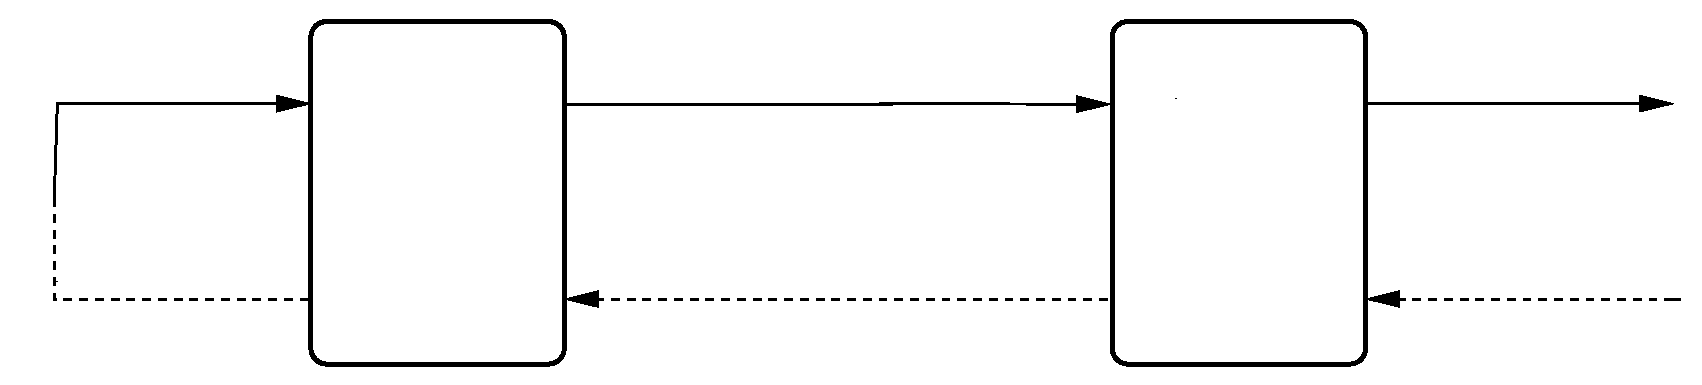
\includegraphics{sc/2node}%
\end{picture}%
\setlength{\unitlength}{4144sp}%
%
\begingroup\makeatletter\ifx\SetFigFont\undefined%
\gdef\SetFigFont#1#2#3#4#5{%
  \reset@font\fontsize{#1}{#2pt}%
  \fontfamily{#3}\fontseries{#4}\fontshape{#5}%
  \selectfont}%
\fi\endgroup%
\begin{picture}(10914,2274)(1114,-4123)
\put(1936,-3796){\makebox(0,0)[lb]{\smash{{\SetFigFont{12}{14.4}{\familydefault}{\mddefault}{\updefault}{\color[rgb]{0,0,0}$S_{2p}(k)$}%
}}}}
\put(11116,-3841){\makebox(0,0)[lb]{\smash{{\SetFigFont{12}{14.4}{\familydefault}{\mddefault}{\updefault}{\color[rgb]{0,0,0}$dem_{1c}(k)$}%
}}}}
\put(1576,-2266){\makebox(0,0)[lb]{\smash{{\SetFigFont{12}{14.4}{\familydefault}{\mddefault}{\updefault}{\color[rgb]{0,0,0}$S_{2p}(k-\tau_M)$}%
}}}}
\put(3106,-2986){\makebox(0,0)[lb]{\smash{{\SetFigFont{14}{16.8}{\familydefault}{\mddefault}{\updefault}{\color[rgb]{0,0,0}Manufacturer}%
}}}}
\put(8641,-2986){\makebox(0,0)[lb]{\smash{{\SetFigFont{14}{16.8}{\familydefault}{\mddefault}{\updefault}{\color[rgb]{0,0,0}Retailer}%
}}}}
\put(6166,-2491){\makebox(0,0)[lb]{\smash{{\SetFigFont{10}{12.0}{\familydefault}{\mddefault}{\updefault}{\color[rgb]{0,0,0}$\tau_T=2$}%
}}}}
\put(1171,-3031){\makebox(0,0)[lb]{\smash{{\SetFigFont{10}{12.0}{\familydefault}{\mddefault}{\updefault}{\color[rgb]{0,0,0}$\tau_M = 2$}%
}}}}
\put(8686,-3301){\makebox(0,0)[lb]{\smash{{\SetFigFont{12}{14.4}{\familydefault}{\mddefault}{\updefault}{\color[rgb]{0,0,0}Node $1$}%
}}}}
\put(9991,-2311){\makebox(0,0)[lb]{\smash{{\SetFigFont{12}{14.4}{\familydefault}{\mddefault}{\updefault}{\color[rgb]{0,0,0}$S_{1c}(k)$}%
}}}}
\put(7201,-3886){\makebox(0,0)[lb]{\smash{{\SetFigFont{12}{14.4}{\familydefault}{\mddefault}{\updefault}{\color[rgb]{0,0,0}$O_{12}(k)$}%
}}}}
\put(4816,-2716){\makebox(0,0)[lb]{\smash{{\SetFigFont{12}{14.4}{\familydefault}{\mddefault}{\updefault}{\color[rgb]{0,0,0}$S_{21}(k)$}%
}}}}
\put(3421,-3301){\makebox(0,0)[lb]{\smash{{\SetFigFont{12}{14.4}{\familydefault}{\mddefault}{\updefault}{\color[rgb]{0,0,0}Node $2$}%
}}}}
\end{picture}%
}
  \end{figure}
 \begin{itemize}
  \item Transportation delay: 2time unit. Manufacturing delay: 2 time units.
  \item {\alert{{Economic control objective}: Minimize operating cost
    \begin{multline*}\ell_E(x,u) = \text{Inventory holding cost}  \\+ \text{Production and Shipping cost} + \text{Lost order/sales cost} \end{multline*}}}
   \item {\color{gray}{{Distributed tracking control objective}: Cooperatively minimize tracking cost
      \[ \ell_T(x,u;z_p) = \norm{x-x_{\text{safety}}}_Q^2 + \norm{u-u_{\text{safety}}}_R^2\]}}
  \item \alert{Nominal demand}: 8 units every time period. 
 \end{itemize}
\end{frame}



\begin{frame}[t]{Two node supply chain example}
\begin{columns}[T]
\column{0.3\textwidth}
{\small{
\begin{gather*}
\min_{\bu} \sum_{i=0}^{N-1} \ell_E(x,u) \\
\text{s.t.~} x^+ = Ax + Bu + B_dd \\
\underline{x} \leq x \leq \overline{x} \\
\underline{u} \leq u \leq \overline{u}
\end{gather*}}}
\column{0.7\textwidth}
\begin{figure}
   \centering
   \resizebox{1\columnwidth}{!}{\input{unstable_SC}}
  \end{figure}
\end{columns}
\begin{itemize}
\item \alert{Economic control objective}
{\small{\begin{multline*}\ell_E(x,u) = \text{Inventory holding cost}+ \text{Production and Shipping cost} +\\ \text{Lost order/sales cost} \end{multline*}}}
  \item Pathological cost : $ \text{Shipping costs} > \text{Lost order
      penalties}$ 
  \item \alert{Controller decides to not meet demand even though costs escalate \ldots} % 
  \newline{\color{blue}{ yet there is a {\em{cheap}} steady state that
      satisfies demands}}
  %\item \alert{Myopic online optimization}
 \end{itemize}
\end{frame}

\begin{frame}{Steady state}
{\tiny{
\begin{multline*}
\underbrace{\begin{bmatrix}\Inv_1\\\BO_1\\\Inv_2 \\
    \BO_2\end{bmatrix}_{k+1}}_{x(k+1)} = 
\underbrace{\begin{bmatrix} 1 & & &
 \\ & 1 & &\\ & & 1 & \\ & & & 1\end{bmatrix}}_{A}
\underbrace{\begin{bmatrix}\Inv_1\\\BO_1\\\Inv_2 \\
    \BO_2\end{bmatrix}_{k}}_{x(k)}+
\underbrace{\begin{bmatrix}-1&0 &0 &0 \\-1&0 &0 &0 \\
0&0 & -1 &0 \\0 & 1 & -1 &0 \end{bmatrix}}_{B}
\underbrace{\begin{bmatrix}S_{1c}\\O_{12}\\S_{21}\\S_{2m}\end{bmatrix}_{k}}_{u(k)}+\\
\underbrace{\begin{bmatrix} 0&0 &1 &0 \\0 &0 &0 &0 \\
0&0 &0  &1 \\0 & 0 &0  &0 \end{bmatrix}}_{B^{(2)}} 
\underbrace{\begin{bmatrix}S_{1c}\\O_{12}\\S_{21}\\S_{2m}\end{bmatrix}_{k-2}}_{u(k-2)}+
\underbrace{\begin{bmatrix}0 \\ 1 \\0 \\0 \end{bmatrix}}_{B_d}\underbrace{\begin{bmatrix}\Dem_{1c}\end{bmatrix}_{k}}_{d(k)}
\end{multline*}}}
\begin{itemize}
\item  All flows in the supply chain are balanced (function of demand)
\[ B^{(2)}u + Bu = -B_dd\]
\item Inventories stabilized at any level; Backorders at zero
\end{itemize}
\end{frame}

{\FooterCite{\citet{rawlings:mayne:2009}}
\begin{frame}{Stability theory: Optimal MPC}
\begin{itemize} 
\item \alert{Cost function}: \qquad $\displaystyle V_N = \sum_{j=0}^{N-1}
  \underbrace{\ell(x(j), u(j))}_{\text{positive semi-definite stage cost}} + \alert{V_f(x(N))}$
\item \alert{Optimization}: \qquad $\displaystyle \min_{\bu} V_N (\bu,
  x(0)) $\\
subject to: \\
\centerline{$\bu = \{u(0), u(1), \ldots u(N-1)\}$}
\centerline{$x^+=Ax+Bu$ \qquad   $\alert{x(N) \in \mathbb{X}_f}$  \qquad $\bu \in \mathbb{U}^N$} 
\item \alert{Closed-loop dynamics}: $x^+ = Ax+ Bu^0(x)$
\item Then, we can show that the \alert{optimal cost $V_N^0(x)$ is a
  Lyapunov function}
\begin{equation*}
V_N^0(x^+)-V_N^0(x) \leq -\alpha(\norm{x}) \qquad \text{cost decrease}
\end{equation*}
\item {\color{blue}{Terminal region + penalty used to approximate
      infinite horizon cost}}
%\item {\color{blue}{Terminal region $\mathbb{X}_f$ ensures recursive feasibility}}
\item {\color{blue}{Lyapunov theory ensures closed-loop
    stability, asymptotic convergence to origin, and more\ldots}}
\end{itemize}
\end{frame}
}

{\FooterCite{\citet{amrit:rawlings:angeli:2011,diehl:amrit:rawlings:2011}}
\begin{frame}{Economic MPC}
\begin{itemize}
\item Uses an economic stage cost
\item {\alert{Unique steady-state}}: \[\min_{x,u}{\ell_E(x,u)} \qquad
    \text{s.t~} x = Ax+Bu, x \in \mathbb{X}, u \in \mathbb{U}\]  
\item {\alert{Strict dissipativity}}: $\exists$ {\em{some}} economic control law.  
\item {\alert{Positive invariant terminal set}}: $\exists$
    $\mathbb{X}_f$ containing the steady state and a {\em{stabilizing}} control law $u = \kappa_f(x)$ that can be {\em{switched on}} in the terminal region.
%\begin{enumerate}
%\item Add terminal cost: $ \displaystyle V_N(x) = V_N = \sum_{j=0}^{N-1}
%  \ell_E(x(j), u(j)) + {\color{blue}{V_f(x(N))}}$
%\item Terminate at steady state:
%{\color{blue}{$\displaystyle \mathbb{X}_f = \set{x_s}$}}  
%\item Terminate in region where the linear feedback controller $u=Kx$ is stabilizing
%{\color{blue}{\begin{equation*} \mathbb{X}_f = \lbrace x \mid x^+ = (A+BK)x \in \mathbb{X}, Kx \in \mathbb{U}, (A+BK) \text{is stable} \rbrace \end{equation*}}}
%\end{enumerate}
\item Use rotated cost function to prove Lyapunov stability
\item {\color{blue}{ Design guidelines to stabilize closed-loop for
    systems optimizing process economics}}
\end{itemize}
\end{frame}
}

\begin{frame}[t]{Two node supply chain example revisited}
\begin{columns}[T]
\column{0.3\textwidth}
{\small{
\begin{gather*}
\min_{\bu} \sum_{i=0}^{N-1} \ell_E(x,u) \\
\text{s.t.~} x^+ = Ax + Bu + B_dd \\
\underline{x} \leq x \leq \overline{x} \\
\underline{u} \leq u \leq \overline{u} \\
\alert{x(N) = x_s} 
\end{gather*}}}
\column{0.7\textwidth}
\begin{figure}
   \centering
   \resizebox{1\columnwidth}{!}{\input{stable_SC}}
  \end{figure}
\end{columns}
\begin{itemize} 
\item \alert{Economic control objective}
{{\begin{multline*}\ell_E(x,u) = \text{Inventory holding cost}+ \text{Production and Shipping cost} \\+ \text{Lost order/sales cost} \end{multline*}}}
  \item Pathological cost : $ \text{Shipping costs} > \text{Lost order
      penalties}$ 
  \item \alert{Controller stabilizes the ``economic'' steady state}
 \end{itemize}
\end{frame}

\begin{frame}{Multiobjective stage cost}
\begin{itemize} 
\item In economic MPC, the stage cost \alert{determines the steady state}
\item {\color{blue}{What if the economic steady state is not the
    desired steady state}}
 \begin{itemize}
  \item In the previous example, steady state inventories were zero
 \end{itemize}
\item Supply chain managers wish to \alert{minimize cost} as well as
  \alert{minimize risk}
\item One way to minimize risk is to \alert{operate around a safety
    stock}
\item \alert{Multiobjective stage cost}
{{ \[ \ell(x,u) = \frac{\omega}{s_E}\ell_E(x,u) +
    \frac{1-\omega}{s_T} \ell_T(x,u;z_p) \]}}
\item $\ell_T(x,u;z_p) = \norm{x-x_{\text{safety}}}_Q^2 +
  \norm{u-u_{\text{safety}}}_R^2$
\item $\omega = 0$: Risk averse; $\omega = 1$: Risk seeking
\end{itemize}
\end{frame}

\begin{frame}{Closed-loop performance}
%\alert{Design Economic MPC  for multiobjective
%   stage cost}
 \begin{figure}
   \centering
   \resizebox{0.9\textwidth}{!}{\input{CL4}}
  \end{figure}
\begin{itemize}
 \item Steady state stabilized depends on choice of $\omega$.  
 \item For $\omega = 0.4$, Multiobjective MPC is $1.75\%$ less
   expensive than tracking MPC to the same steady state!
\begin{itemize}
 \item {\color{blue}{Knowledge of economics in the cost function means that
   economically attractive transients are preferred}}  
\end{itemize}
\item Pure economic MPC ($\omega = 1)$ cannot even stabilize the
  steady state for the
   initial conditions chosen.
\begin{itemize}
 \item Can design larger region of attraction for multiobjective stage cost
\end{itemize}
\end{itemize}
\end{frame}
{\NoHeaderFooter
\begin{frame}{Outline-I}
\addtocounter{framenumber}{-1}
\begin{itemize}
 \item {{Detailed optimization model + rolling horizon guarantees \ldots \\ 
 \centerline{{no reasonable closed-loop properties!}}}}
 \item Examples:
 \begin{enumerate}
  \item {\color{gray}{Supply chain minimizing costs does not meet customer demands}}
  {\alert{ \item Manufacturing facility cannot find feasible schedules }}
 \end{enumerate} 
% \end{itemize}
%\end{exampleblock} 
%\begin{block}{}
% \begin{itemize}
  \item Rolling horizon + MPC design guarantees
    \ldots \\ 
  \centerline{{favorable closed-loop properties like stability, convergence.}} 
  \item Contributions:
  \begin{enumerate}
   
   \item {\color{gray}{Stability and convergence guarantees for supply
         chain using Economic MPC}}
   {\alert{
   \item {{Recursive feasibility and rescheduling
         techniques for iterative scheduling}}
     }}
  \end{enumerate}
 \end{itemize}
\end{frame}
}

{\FooterCite{\citet{subramanian:maravelias:rawlings:2012}}
\begin{frame}[t]{State space model for chemical production scheduling}
\begin{columns}[T]
\column{0.6\textwidth}
\begin{figure}
  \centering
  \resizebox{0.5\columnwidth}{!}{\begin{picture}(0,0)%
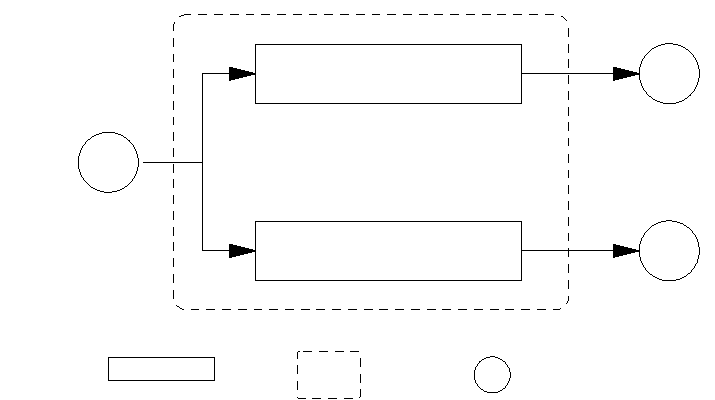
\includegraphics{scheduling/ABexample}%
\end{picture}%
\setlength{\unitlength}{4144sp}%
%
\begingroup\makeatletter\ifx\SetFigFont\undefined%
\gdef\SetFigFont#1#2#3#4#5{%
  \reset@font\fontsize{#1}{#2pt}%
  \fontfamily{#3}\fontseries{#4}\fontshape{#5}%
  \selectfont}%
\fi\endgroup%
\begin{picture}(5430,3041)(76,-3447)
\put( 91,-1726){\makebox(0,0)[lb]{\smash{{\SetFigFont{17}{20.4}{\rmdefault}{\mddefault}{\updefault}{\color[rgb]{0,.56,0}RM}%
}}}}
\put(3061,-3301){\makebox(0,0)[lb]{\smash{{\SetFigFont{17}{20.4}{\rmdefault}{\mddefault}{\updefault}{\color[rgb]{0,0,0}Unit}%
}}}}
\put(4141,-3301){\makebox(0,0)[lb]{\smash{{\SetFigFont{17}{20.4}{\rmdefault}{\mddefault}{\updefault}{\color[rgb]{0,0,0}Material}%
}}}}
\put(1801,-3301){\makebox(0,0)[lb]{\smash{{\SetFigFont{17}{20.4}{\rmdefault}{\mddefault}{\updefault}{\color[rgb]{0,0,0}Task}%
}}}}
\put(2971,-1051){\makebox(0,0)[lb]{\smash{{\SetFigFont{17}{20.4}{\rmdefault}{\mddefault}{\updefault}{\color[rgb]{0,0,0}TA}%
}}}}
\put(2971,-2401){\makebox(0,0)[lb]{\smash{{\SetFigFont{17}{20.4}{\rmdefault}{\mddefault}{\updefault}{\color[rgb]{0,0,0}TB}%
}}}}
\put(1126,-556){\makebox(0,0)[lb]{\smash{{\SetFigFont{17}{20.4}{\rmdefault}{\mddefault}{\updefault}{\color[rgb]{0,0,0}U}%
}}}}
\put(1801,-1996){\makebox(0,0)[lb]{\smash{{\SetFigFont{17}{20.4}{\rmdefault}{\mddefault}{\updefault}{\color[rgb]{0,0,0}$\tau_{TB}=2$hr, $\beta_{TB}=6$ton}%
}}}}
\put(1801,-1411){\makebox(0,0)[lb]{\smash{{\SetFigFont{17}{20.4}{\rmdefault}{\mddefault}{\updefault}{\color[rgb]{0,0,0}$\tau_{TA}=3$hr, $\beta_{TA}=4$ton }%
}}}}
\put(5491,-2401){\makebox(0,0)[lb]{\smash{{\SetFigFont{17}{20.4}{\rmdefault}{\mddefault}{\updefault}{\color[rgb]{1,0,0}$B$}%
}}}}
\put(5491,-1006){\makebox(0,0)[lb]{\smash{{\SetFigFont{17}{20.4}{\rmdefault}{\mddefault}{\updefault}{\color[rgb]{0,0,1}$A$}%
}}}}
\end{picture}%
}
  %\caption{Simple scheduling problem}
  %\label{fig:scheduling:ABexample}
\end{figure}
\begin{figure}
  \centering
  \resizebox{0.8\columnwidth}{!}{\input{ABlift0}}
  %\caption{Simple scheduling problem}
  %\label{fig:scheduling:ABexample}
\end{figure}
\column{0.4\textwidth}
\begin{itemize}
\item Inputs: $W_{i,t}$
\item States: $S_{k,t}$
\item At $t=2$ and $t=3$, all the inputs and states are same
\item Need additional states to ``capture'' history of the system
\item \alert{Lifting of task variables}
\end{itemize}
\end{columns}
\end{frame}
}

{\FooterCite{\citet{subramanian:maravelias:rawlings:2012}}
\begin{frame}[t]{Lifting}
\begin{figure}
  \centering
  \resizebox{0.7\columnwidth}{!}{\begin{picture}(0,0)%
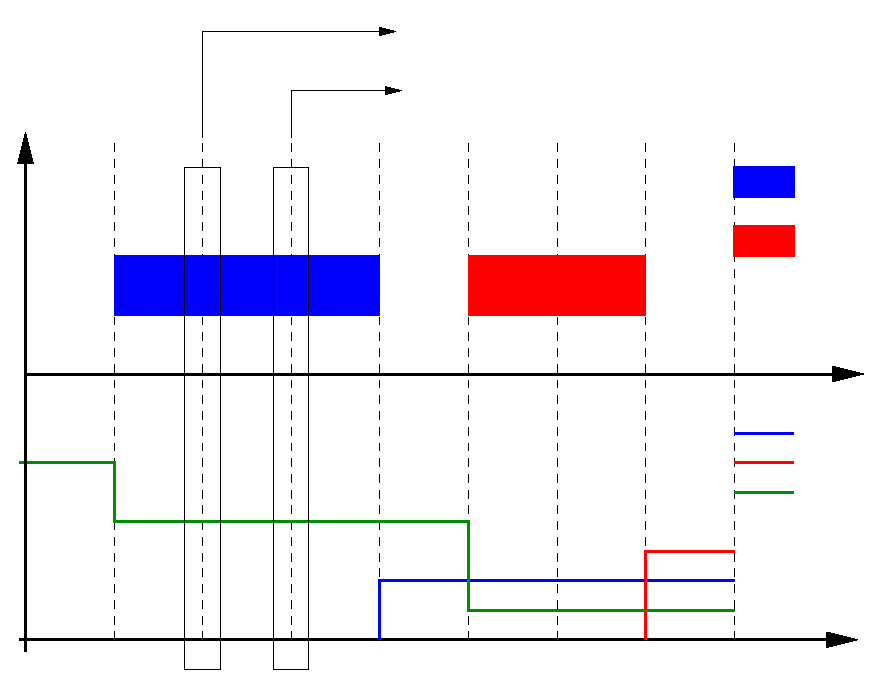
\includegraphics{ABlift1}%
\end{picture}%
\setlength{\unitlength}{4144sp}%
%
\begingroup\makeatletter\ifx\SetFigFont\undefined%
\gdef\SetFigFont#1#2#3#4#5{%
  \reset@font\fontsize{#1}{#2pt}%
  \fontfamily{#3}\fontseries{#4}\fontshape{#5}%
  \selectfont}%
\fi\endgroup%
\begin{picture}(6479,4977)(1959,-5476)
\put(4951,-1051){\makebox(0,0)[lb]{\smash{{\SetFigFont{14}{16.8}{\rmdefault}{\mddefault}{\updefault}{\color[rgb]{0,0,0}$W_{\text{TA},3}=0,W_{\text{TB},3}=0,S_{\text{RM},3}=8,S_{A,3}=S_{B,3}=0,$\alert{$\bar{W}_{\text{TA},3}^2=1$}}%
}}}}
\put(7966,-3706){\makebox(0,0)[lb]{\smash{{\SetFigFont{17}{20.4}{\rmdefault}{\mddefault}{\updefault}{\color[rgb]{0,0,0}$S_{A,t}$}%
}}}}
\put(7966,-3931){\makebox(0,0)[lb]{\smash{{\SetFigFont{17}{20.4}{\rmdefault}{\mddefault}{\updefault}{\color[rgb]{0,0,0}$S_{B,t}$}%
}}}}
\put(7966,-4156){\makebox(0,0)[lb]{\smash{{\SetFigFont{17}{20.4}{\rmdefault}{\mddefault}{\updefault}{\color[rgb]{0,0,0}$S_{RM,t}$}%
}}}}
\put(7831,-5461){\makebox(0,0)[lb]{\smash{{\SetFigFont{17}{20.4}{\rmdefault}{\mddefault}{\updefault}{\color[rgb]{0,0,0}Time}%
}}}}
\put(3376,-5416){\makebox(0,0)[lb]{\smash{{\SetFigFont{17}{20.4}{\rmdefault}{\mddefault}{\updefault}{\color[rgb]{0,0,0}2}%
}}}}
\put(4726,-5416){\makebox(0,0)[lb]{\smash{{\SetFigFont{17}{20.4}{\rmdefault}{\mddefault}{\updefault}{\color[rgb]{0,0,0}4}%
}}}}
\put(6076,-5416){\makebox(0,0)[lb]{\smash{{\SetFigFont{17}{20.4}{\rmdefault}{\mddefault}{\updefault}{\color[rgb]{0,0,0}6}%
}}}}
\put(7426,-5416){\makebox(0,0)[lb]{\smash{{\SetFigFont{17}{20.4}{\rmdefault}{\mddefault}{\updefault}{\color[rgb]{0,0,0}8}%
}}}}
\put(8056,-2221){\makebox(0,0)[lb]{\smash{{\SetFigFont{17}{20.4}{\rmdefault}{\mddefault}{\updefault}{\color[rgb]{0,0,0}TB}%
}}}}
\put(8056,-1816){\makebox(0,0)[lb]{\smash{{\SetFigFont{17}{20.4}{\rmdefault}{\mddefault}{\updefault}{\color[rgb]{0,0,0}TA}%
}}}}
\put(4861,-646){\makebox(0,0)[lb]{\smash{{\SetFigFont{14}{16.8}{\rmdefault}{\mddefault}{\updefault}{\color[rgb]{0,0,0}$W_{\text{TA},2}=0,W_{\text{TB},2}=0,S_{\text{RM},2}=8,S_{A,2}=S_{B,2}=0,$\alert{$\bar{W}_{\text{TA},2}^1=1$}}%
}}}}
\end{picture}%
}
  %\caption{Simple scheduling problem}
  %\label{fig:scheduling:ABexample}
\end{figure}
\begin{itemize}
\item Lifted state $\bar{W}_{i,t}^n = 1$ if task $i$ started at $t-n$
\item Lifted state ``dynamics''
\[ \bar{W}_{i,t+1}^n = \bar{W}_{i,t}^{n-1}\]
\end{itemize}
\end{frame}
}

{\FooterCite{\citet{subramanian:maravelias:rawlings:2012}}
\begin{frame}{State space model}
\begin{itemize}
\item \alert{States}: $ x = \begin{bmatrix} S_{k,t} &
    \bar{W}_{i,t}^n \end{bmatrix}$
 \item \alert{Inputs}: $u = \begin{bmatrix} W_{i,t} \end{bmatrix}$
\item \alert{Disturbance}: $d$ are the demands $d = \begin{bmatrix}
    \Dem_{k,t} \end{bmatrix}$
\item \alert{Dynamics}: $x^+ = Ax + Bu + B_dd$:
  \begin{itemize}
    \item Inventory balance
    \item Lifted state dynamics
  \end{itemize}
\item \alert{Constraints}:
  \begin{itemize}
    \item  Resource allocation constraint is a mixed state-input
      constraint
     \item Input constraints $W_{i,t} \in \set{0,1}$
     \item State constraints $S_{k,t} \in [0,\sigma_k]$
   \end{itemize}
\item {\color{blue}{Can be generalized to model variable batch size,
    changeovers, etc.}}
\end{itemize}
\end{frame}
}

\begin{frame}[t]{Rolling horizon optimization}
\begin{columns}[T]
\column{0.2\textwidth}
{\tiny{
 \begin{gather*}
\min_{\bu} \sum_{i=0}^{N-1} \ell_E(x,u) \\
\text{s.t.~} x^+ = Ax + Bu + B_dd \\
\underline{x} \leq x \leq \overline{x} \\
\underline{u} \leq u \leq \overline{u}
\end{gather*}}}
\column{0.8\textwidth}
\begin{figure}
   %\centering
   \includegraphics[scale=0.65]{gantt_NT.pdf}
  \end{figure}
\end{columns}
\begin{itemize} 
\item \alert{1 unit, 2 tasks with changeover times and variable batch sizes}
\item Infeasible at time $t=2$ because batch started at $t=1$ (6 tons) is too
  small when new demand at $t=2+N$ is observed.
\item {\color{blue}{Can terminal constraints be used?}}
\end{itemize}
\end{frame}

\begin{frame}{Periodic solution}
\begin{columns}[T]
\column{0.3\textwidth}
{\tiny{
 \begin{gather*}
\min_{\bu,x(0)} \sum_{i=0}^{N_p-1} \ell_E(x,u) \\
\text{s.t.~} x^+ = Ax + Bu + B_dd \\
\underline{x} \leq x \leq \overline{x} \\
\underline{u} \leq u \leq \overline{u} \\
\alert{x(0) = x(N_p)}
\end{gather*}}}
\column{0.7\textwidth}
\begin{figure}
   %\centering
   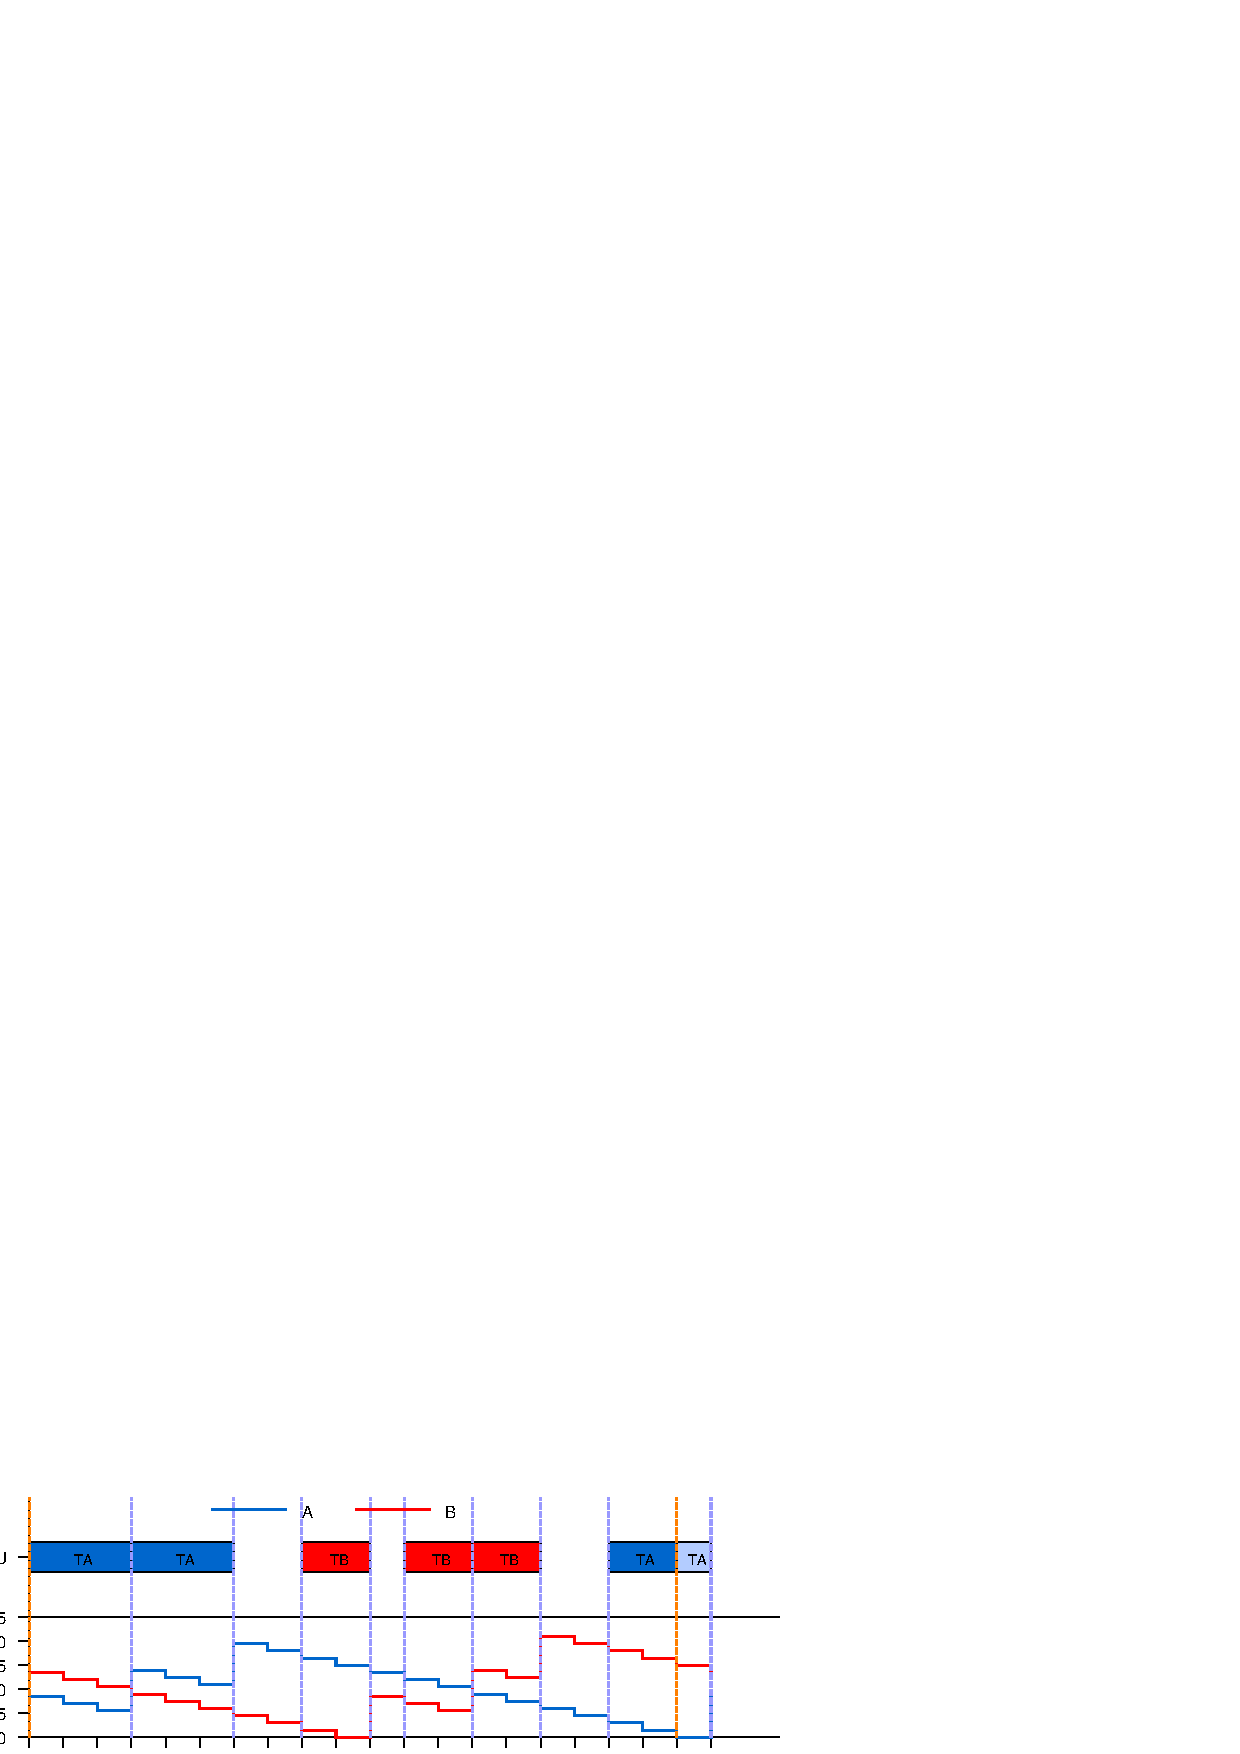
\includegraphics[scale=0.45]{gantt_Periodic.pdf}
  \end{figure}
\end{columns} 
\centerline{\color{blue}{A suboptimal infinite
    horizon solution in response to nominal demands}}
 
\begin{columns}[T]
\column{0.3\textwidth}
{\tiny{
 \begin{gather*}
\min_{\bu} \sum_{i=0}^{N-1} \ell_E(x,u) \\
\text{s.t.~} x^+ = Ax + Bu + B_dd \\
\underline{x} \leq x \leq \overline{x} \\
\underline{u} \leq u \leq \overline{u} \\
\alert{x(N) = \text{A state on the periodic profile}}
\end{gather*}}}
\column{0.7\textwidth}
\begin{figure}
   %\centering
   \includegraphics[scale=0.30]{gantt_24.pdf}
  \end{figure}
\end{columns}
\centerline{\color{blue}{Observe that batch size at $t=1$ is 8.5 tons}}
\end{frame}

\begin{frame}{Modeling disturbances}
\begin{itemize} 
\item \alert{Rescheduling}\footnote{\citet{li:ierapetritou:2008b}}
 \begin{itemize}
   \item When unplanned events (like breakdown, loading error) occurs
   \item Local corrections: Repair solution within the same
     scheduling horizon (\alert{Scheduling as a static problem})
   \item Heuristic corrections
   \item Parametric programming
   \item Stochastic programming
 \end{itemize}
\item MPC provides a natural framework for rescheduling
  \begin{itemize}
    \item Solve optimization problem based on ``feedback'' from
      process
   \item Rolling horizon could lead to better solutions
     (\alert{Scheduling as a dynamic problem})
  \end{itemize}
\item {\color{blue}{Model events that can lead to rescheduling as disturbances}}
\end{itemize}
\end{frame}

\begin{frame}{$1h$ delay in the task}
\begin{figure}
\centering
 \resizebox{0.65\textwidth}{!}{\begin{picture}(0,0)%
\includegraphics{ABdelay}%
\end{picture}%
\setlength{\unitlength}{4144sp}%
%
\begingroup\makeatletter\ifx\SetFigFont\undefined%
\gdef\SetFigFont#1#2#3#4#5{%
  \reset@font\fontsize{#1}{#2pt}%
  \fontfamily{#3}\fontseries{#4}\fontshape{#5}%
  \selectfont}%
\fi\endgroup%
\begin{picture}(7012,4257)(1959,-5476)
\put(2251,-1546){\makebox(0,0)[lb]{\smash{{\SetFigFont{20}{24.0}{\rmdefault}{\mddefault}{\updefault}{\color[rgb]{0,0,0}$t=3$}%
}}}}
\put(7831,-5461){\makebox(0,0)[lb]{\smash{{\SetFigFont{17}{20.4}{\rmdefault}{\mddefault}{\updefault}{\color[rgb]{0,0,0}Time}%
}}}}
\put(3376,-5416){\makebox(0,0)[lb]{\smash{{\SetFigFont{17}{20.4}{\rmdefault}{\mddefault}{\updefault}{\color[rgb]{0,0,0}2}%
}}}}
\put(4726,-5416){\makebox(0,0)[lb]{\smash{{\SetFigFont{17}{20.4}{\rmdefault}{\mddefault}{\updefault}{\color[rgb]{0,0,0}4}%
}}}}
\put(6076,-5416){\makebox(0,0)[lb]{\smash{{\SetFigFont{17}{20.4}{\rmdefault}{\mddefault}{\updefault}{\color[rgb]{0,0,0}6}%
}}}}
\put(7426,-5416){\makebox(0,0)[lb]{\smash{{\SetFigFont{17}{20.4}{\rmdefault}{\mddefault}{\updefault}{\color[rgb]{0,0,0}8}%
}}}}
\put(8056,-2221){\makebox(0,0)[lb]{\smash{{\SetFigFont{17}{20.4}{\rmdefault}{\mddefault}{\updefault}{\color[rgb]{0,0,0}TB}%
}}}}
\put(8056,-1816){\makebox(0,0)[lb]{\smash{{\SetFigFont{17}{20.4}{\rmdefault}{\mddefault}{\updefault}{\color[rgb]{0,0,0}TA}%
}}}}
\put(2296,-3661){\makebox(0,0)[lb]{\smash{{\SetFigFont{20}{24.0}{\rmdefault}{\mddefault}{\updefault}{\color[rgb]{0,0,0}$t=4$}%
}}}}
\put(8956,-1501){\makebox(0,0)[lb]{\smash{{\SetFigFont{14}{16.8}{\rmdefault}{\mddefault}{\updefault}{\color[rgb]{0,0,0}$\bar{W}_{\text{TA},3}^2 = 1$}%
}}}}
\put(8821,-3481){\makebox(0,0)[lb]{\smash{{\SetFigFont{14}{16.8}{\rmdefault}{\mddefault}{\updefault}{\color[rgb]{0,0,0}$\bar{W}_{\text{TA},4}^3 = 1 \rightarrow \bar{W}_{\text{TA},4}^3 = 0$}%
}}}}
\put(8821,-3751){\makebox(0,0)[lb]{\smash{{\SetFigFont{14}{16.8}{\rmdefault}{\mddefault}{\updefault}{\color[rgb]{0,0,0}$\bar{W}_{\text{TA},4}^2 = 0 \rightarrow \bar{W}_{\text{TA},4}^2 = 1$}%
}}}}
\put(2206,-1366){\makebox(0,0)[lb]{\smash{{\SetFigFont{20}{24.0}{\rmdefault}{\mddefault}{\updefault}{\color[rgb]{0,0,0}$1h$ delay is observed}%
}}}}
\end{picture}%
}
\end{figure}
\begin{itemize}
\item Disturbance variable $\hat{Y}_{i,t}^n = 1$ if $1h$ delay in task
  $i$ is observed

\item \alert{Lifted dynamics correction}:
  \[ \bar{W}_{i,t+1}^{n} = \bar{W}_{i,t}^{n-1} + \hat{Y}_{i,t}^{n} -
\hat{Y}_{i,t}^{n-1}\]
\item Similarly we can write \alert{inventory correction}
\item $d = \begin{bmatrix} \Dem_{k,t} & \hat{Y}_{i,t}^n \end{bmatrix}$
\end{itemize}
\end{frame}

\begin{frame}{Rescheduling}
\begin{figure}
   %\centering
   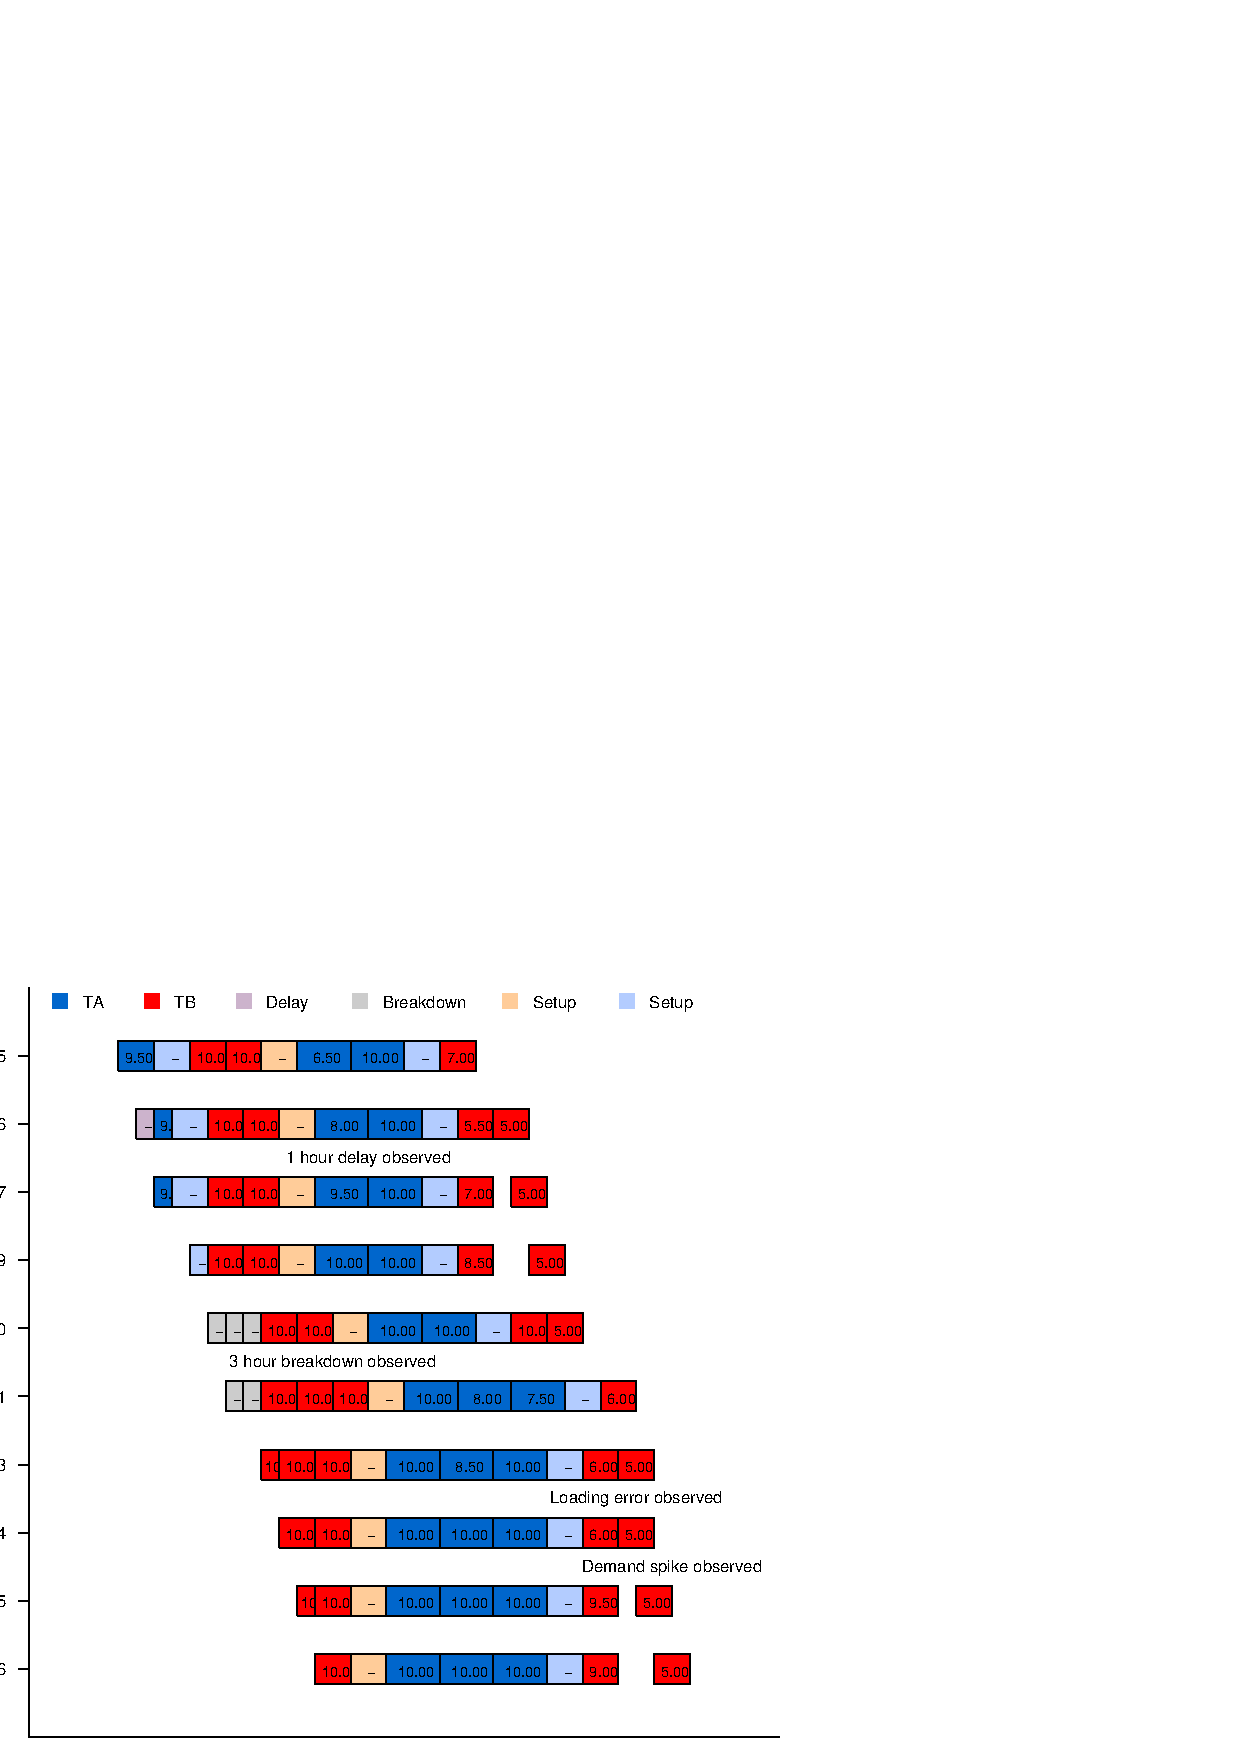
\includegraphics[scale=0.4]{gantt_NT_disturbance.pdf}
  \end{figure}
\end{frame}

\begin{frame}{Multi-product, multi-echelon supply chain example}
\begin{figure}
\centering
\scriptsize
\resizebox{0.5\textwidth}{!}{\begin{picture}(0,0)%
\includegraphics{sc/lssc}%
\end{picture}%
\setlength{\unitlength}{4144sp}%
%
\begingroup\makeatletter\ifx\SetFigFont\undefined%
\gdef\SetFigFont#1#2#3#4#5{%
  \reset@font\fontsize{#1}{#2pt}%
  \fontfamily{#3}\fontseries{#4}\fontshape{#5}%
  \selectfont}%
\fi\endgroup%
\begin{picture}(10101,6366)(1363,-5719)
\put(10801,164){\makebox(0,0)[lb]{\smash{{\SetFigFont{17}{20.4}{\familydefault}{\mddefault}{\updefault}{\color[rgb]{0,0,0}$R1$}%
}}}}
\put(2071,-2851){\makebox(0,0)[lb]{\smash{{\SetFigFont{17}{20.4}{\familydefault}{\mddefault}{\updefault}{\color[rgb]{0,0,0}$M1$}%
}}}}
\put(7246,-736){\makebox(0,0)[lb]{\smash{{\SetFigFont{17}{20.4}{\familydefault}{\mddefault}{\updefault}{\color[rgb]{0,0,0}$D1$}%
}}}}
\put(7291,-4741){\makebox(0,0)[lb]{\smash{{\SetFigFont{17}{20.4}{\familydefault}{\mddefault}{\updefault}{\color[rgb]{0,0,0}$D2$}%
}}}}
\put(10801,-5371){\makebox(0,0)[lb]{\smash{{\SetFigFont{17}{20.4}{\familydefault}{\mddefault}{\updefault}{\color[rgb]{0,0,0}$R4$}%
}}}}
\put(10846,-4111){\makebox(0,0)[lb]{\smash{{\SetFigFont{17}{20.4}{\familydefault}{\mddefault}{\updefault}{\color[rgb]{0,0,0}$R3$}%
}}}}
\put(10801,-1231){\makebox(0,0)[lb]{\smash{{\SetFigFont{17}{20.4}{\familydefault}{\mddefault}{\updefault}{\color[rgb]{0,0,0}$R2$}%
}}}}
\end{picture}%
}
\end{figure}
\begin{itemize}
\item Two products $A$ \& $B$ handled by each node.
\item \alert{Example 1}: Independent units for production;\\
  {\color{blue}{Multiobjective stage cost}}
\item \alert{Example 2}: Shared unit for production;\\
  {\color{blue}{Integrated scheduling and inventory control}}
\end{itemize}
\end{frame} 
\begin{frame}
\frametitle{Comparison with other operating policies}
\alert{$(\sigma,\Sigma)$ operating policy:}
 \begin{itemize}
   \item Order $\Sigma-\sigma$ if inventory falls below $\sigma$.
   \item If Inventory is available, meet all demands.
 \end{itemize}
\alert{Bullwhip effect}: In this study, the bullwhip effect is
  quantified as the increase in variance of the orders placed as we
  move upstream in the supply chain.
\end{frame}
\begin{frame}{Results}
\begin{figure}
\centering 
\scriptsize
\resizebox{0.75\textwidth}{!}{% GNUPLOT: LaTeX picture with Postscript
\begingroup
  \makeatletter
  \providecommand\color[2][]{%
    \GenericError{(gnuplot) \space\space\space\@spaces}{%
      Package color not loaded in conjunction with
      terminal option `colourtext'%
    }{See the gnuplot documentation for explanation.%
    }{Either use 'blacktext' in gnuplot or load the package
      color.sty in LaTeX.}%
    \renewcommand\color[2][]{}%
  }%
  \providecommand\includegraphics[2][]{%
    \GenericError{(gnuplot) \space\space\space\@spaces}{%
      Package graphicx or graphics not loaded%
    }{See the gnuplot documentation for explanation.%
    }{The gnuplot epslatex terminal needs graphicx.sty or graphics.sty.}%
    \renewcommand\includegraphics[2][]{}%
  }%
  \providecommand\rotatebox[2]{#2}%
  \@ifundefined{ifGPcolor}{%
    \newif\ifGPcolor
    \GPcolorfalse
  }{}%
  \@ifundefined{ifGPblacktext}{%
    \newif\ifGPblacktext
    \GPblacktexttrue
  }{}%
  % define a \g@addto@macro without @ in the name:
  \let\gplgaddtomacro\g@addto@macro
  % define empty templates for all commands taking text:
  \gdef\gplbacktext{}%
  \gdef\gplfronttext{}%
  \makeatother
  \ifGPblacktext
    % no textcolor at all
    \def\colorrgb#1{}%
    \def\colorgray#1{}%
  \else
    % gray or color?
    \ifGPcolor
      \def\colorrgb#1{\color[rgb]{#1}}%
      \def\colorgray#1{\color[gray]{#1}}%
      \expandafter\def\csname LTw\endcsname{\color{white}}%
      \expandafter\def\csname LTb\endcsname{\color{black}}%
      \expandafter\def\csname LTa\endcsname{\color{black}}%
      \expandafter\def\csname LT0\endcsname{\color[rgb]{1,0,0}}%
      \expandafter\def\csname LT1\endcsname{\color[rgb]{0,1,0}}%
      \expandafter\def\csname LT2\endcsname{\color[rgb]{0,0,1}}%
      \expandafter\def\csname LT3\endcsname{\color[rgb]{1,0,1}}%
      \expandafter\def\csname LT4\endcsname{\color[rgb]{0,1,1}}%
      \expandafter\def\csname LT5\endcsname{\color[rgb]{1,1,0}}%
      \expandafter\def\csname LT6\endcsname{\color[rgb]{0,0,0}}%
      \expandafter\def\csname LT7\endcsname{\color[rgb]{1,0.3,0}}%
      \expandafter\def\csname LT8\endcsname{\color[rgb]{0.5,0.5,0.5}}%
    \else
      % gray
      \def\colorrgb#1{\color{black}}%
      \def\colorgray#1{\color[gray]{#1}}%
      \expandafter\def\csname LTw\endcsname{\color{white}}%
      \expandafter\def\csname LTb\endcsname{\color{black}}%
      \expandafter\def\csname LTa\endcsname{\color{black}}%
      \expandafter\def\csname LT0\endcsname{\color{black}}%
      \expandafter\def\csname LT1\endcsname{\color{black}}%
      \expandafter\def\csname LT2\endcsname{\color{black}}%
      \expandafter\def\csname LT3\endcsname{\color{black}}%
      \expandafter\def\csname LT4\endcsname{\color{black}}%
      \expandafter\def\csname LT5\endcsname{\color{black}}%
      \expandafter\def\csname LT6\endcsname{\color{black}}%
      \expandafter\def\csname LT7\endcsname{\color{black}}%
      \expandafter\def\csname LT8\endcsname{\color{black}}%
    \fi
  \fi
  \setlength{\unitlength}{0.0500bp}%
  \begin{picture}(7200.00,5040.00)%
    \gplgaddtomacro\gplbacktext{%
      \csname LTb\endcsname%
      \put(946,846){\makebox(0,0)[r]{\strut{} 0}}%
      \put(946,1828){\makebox(0,0)[r]{\strut{} 0.5}}%
      \put(946,2811){\makebox(0,0)[r]{\strut{} 1}}%
      \put(946,3793){\makebox(0,0)[r]{\strut{} 1.5}}%
      \put(946,4775){\makebox(0,0)[r]{\strut{} 2}}%
      \put(2223,714){\rotatebox{-45}{\makebox(0,0)[l]{\strut{}R1}}}%
      \put(3368,714){\rotatebox{-45}{\makebox(0,0)[l]{\strut{}R5}}}%
      \put(4513,714){\rotatebox{-45}{\makebox(0,0)[l]{\strut{}D1}}}%
      \put(5658,714){\rotatebox{-45}{\makebox(0,0)[l]{\strut{}D2}}}%
      \put(176,2810){\rotatebox{-270}{\makebox(0,0){\strut{}Standard deviation of Orders}}}%
    }%
    \gplgaddtomacro\gplfronttext{%
      \csname LTb\endcsname%
      \put(3085,173){\makebox(0,0)[r]{\strut{}Incoming}}%
      \csname LTb\endcsname%
      \put(4996,173){\makebox(0,0)[r]{\strut{}MPC}}%
    }%
    \gplbacktext
    \put(0,0){\includegraphics{bullwhip}}%
    \gplfronttext
  \end{picture}%
\endgroup
}
\scriptsize
\resizebox{0.75\textwidth}{!}{% GNUPLOT: LaTeX picture with Postscript
\begingroup
  \makeatletter
  \providecommand\color[2][]{%
    \GenericError{(gnuplot) \space\space\space\@spaces}{%
      Package color not loaded in conjunction with
      terminal option `colourtext'%
    }{See the gnuplot documentation for explanation.%
    }{Either use 'blacktext' in gnuplot or load the package
      color.sty in LaTeX.}%
    \renewcommand\color[2][]{}%
  }%
  \providecommand\includegraphics[2][]{%
    \GenericError{(gnuplot) \space\space\space\@spaces}{%
      Package graphicx or graphics not loaded%
    }{See the gnuplot documentation for explanation.%
    }{The gnuplot epslatex terminal needs graphicx.sty or graphics.sty.}%
    \renewcommand\includegraphics[2][]{}%
  }%
  \providecommand\rotatebox[2]{#2}%
  \@ifundefined{ifGPcolor}{%
    \newif\ifGPcolor
    \GPcolorfalse
  }{}%
  \@ifundefined{ifGPblacktext}{%
    \newif\ifGPblacktext
    \GPblacktexttrue
  }{}%
  % define a \g@addto@macro without @ in the name:
  \let\gplgaddtomacro\g@addto@macro
  % define empty templates for all commands taking text:
  \gdef\gplbacktext{}%
  \gdef\gplfronttext{}%
  \makeatother
  \ifGPblacktext
    % no textcolor at all
    \def\colorrgb#1{}%
    \def\colorgray#1{}%
  \else
    % gray or color?
    \ifGPcolor
      \def\colorrgb#1{\color[rgb]{#1}}%
      \def\colorgray#1{\color[gray]{#1}}%
      \expandafter\def\csname LTw\endcsname{\color{white}}%
      \expandafter\def\csname LTb\endcsname{\color{black}}%
      \expandafter\def\csname LTa\endcsname{\color{black}}%
      \expandafter\def\csname LT0\endcsname{\color[rgb]{1,0,0}}%
      \expandafter\def\csname LT1\endcsname{\color[rgb]{0,1,0}}%
      \expandafter\def\csname LT2\endcsname{\color[rgb]{0,0,1}}%
      \expandafter\def\csname LT3\endcsname{\color[rgb]{1,0,1}}%
      \expandafter\def\csname LT4\endcsname{\color[rgb]{0,1,1}}%
      \expandafter\def\csname LT5\endcsname{\color[rgb]{1,1,0}}%
      \expandafter\def\csname LT6\endcsname{\color[rgb]{0,0,0}}%
      \expandafter\def\csname LT7\endcsname{\color[rgb]{1,0.3,0}}%
      \expandafter\def\csname LT8\endcsname{\color[rgb]{0.5,0.5,0.5}}%
    \else
      % gray
      \def\colorrgb#1{\color{black}}%
      \def\colorgray#1{\color[gray]{#1}}%
      \expandafter\def\csname LTw\endcsname{\color{white}}%
      \expandafter\def\csname LTb\endcsname{\color{black}}%
      \expandafter\def\csname LTa\endcsname{\color{black}}%
      \expandafter\def\csname LT0\endcsname{\color{black}}%
      \expandafter\def\csname LT1\endcsname{\color{black}}%
      \expandafter\def\csname LT2\endcsname{\color{black}}%
      \expandafter\def\csname LT3\endcsname{\color{black}}%
      \expandafter\def\csname LT4\endcsname{\color{black}}%
      \expandafter\def\csname LT5\endcsname{\color{black}}%
      \expandafter\def\csname LT6\endcsname{\color{black}}%
      \expandafter\def\csname LT7\endcsname{\color{black}}%
      \expandafter\def\csname LT8\endcsname{\color{black}}%
    \fi
  \fi
  \setlength{\unitlength}{0.0500bp}%
  \begin{picture}(7200.00,3024.00)%
    \gplgaddtomacro\gplbacktext{%
      \csname LTb\endcsname%
      \put(594,946){\makebox(0,0)[r]{\strut{} 0}}%
      \put(594,2155){\makebox(0,0)[r]{\strut{} 10}}%
      \put(828,484){\makebox(0,0){\strut{} 0}}%
      \put(1339,484){\makebox(0,0){\strut{} 10}}%
      \put(1850,484){\makebox(0,0){\strut{} 20}}%
      \put(2361,484){\makebox(0,0){\strut{} 30}}%
      \put(2872,484){\makebox(0,0){\strut{} 40}}%
      \put(3383,484){\makebox(0,0){\strut{} 50}}%
      \put(2054,154){\makebox(0,0){\strut{}Time}}%
    }%
    \gplgaddtomacro\gplfronttext{%
      \csname LTb\endcsname%
      \put(2396,2586){\makebox(0,0)[r]{\strut{}Inventory}}%
      \csname LTb\endcsname%
      \put(2396,2366){\makebox(0,0)[r]{\strut{}Backorder}}%
    }%
    \gplgaddtomacro\gplbacktext{%
      \csname LTb\endcsname%
      \put(4201,484){\makebox(0,0){\strut{} 0}}%
      \put(4661,484){\makebox(0,0){\strut{} 10}}%
      \put(5121,484){\makebox(0,0){\strut{} 20}}%
      \put(5582,484){\makebox(0,0){\strut{} 30}}%
      \put(6042,484){\makebox(0,0){\strut{} 40}}%
      \put(6502,484){\makebox(0,0){\strut{} 50}}%
      \put(6634,704){\makebox(0,0)[l]{\strut{} 0}}%
      \put(6634,1732){\makebox(0,0)[l]{\strut{} 10}}%
      \put(6634,2759){\makebox(0,0)[l]{\strut{} 20}}%
      \put(5305,154){\makebox(0,0){\strut{}Time}}%
    }%
    \gplgaddtomacro\gplfronttext{%
      \csname LTb\endcsname%
      \put(5779,2586){\makebox(0,0)[r]{\strut{}Customer demand}}%
      \csname LTb\endcsname%
      \put(5779,2366){\makebox(0,0)[r]{\strut{}Orders placed}}%
    }%
    \gplbacktext
    \put(0,0){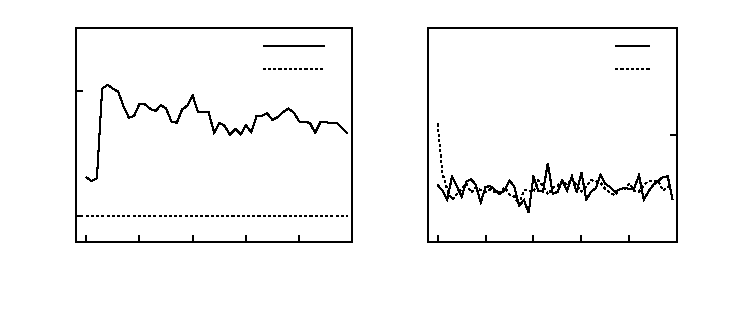
\includegraphics{R3}}%
    \gplfronttext
  \end{picture}%
\endgroup
}
\end{figure}
\end{frame}

\begin{frame}{Integrating scheduling and inventory control}
\begin{figure}
\centering 
  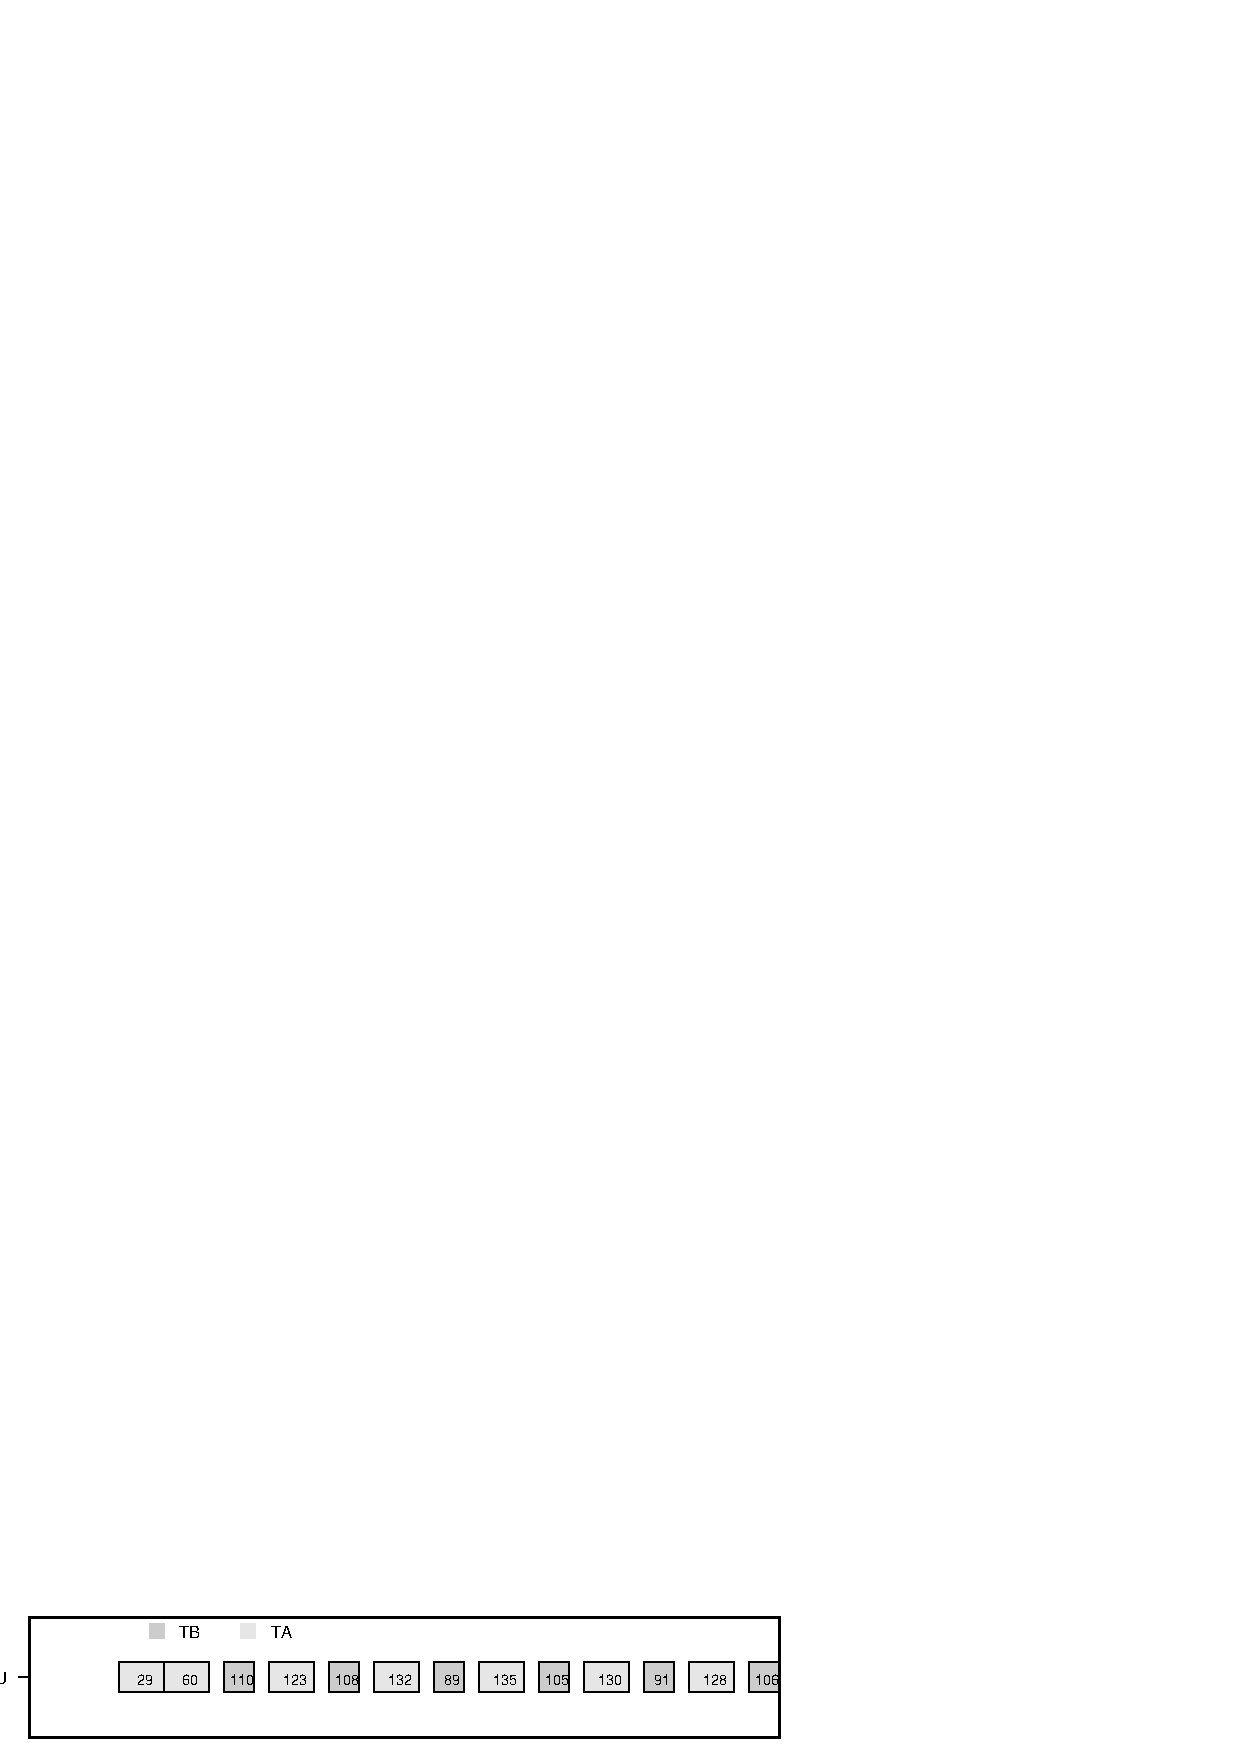
\includegraphics[scale=0.5]{NTS_gantt.pdf}
\end{figure}
\begin{figure}
  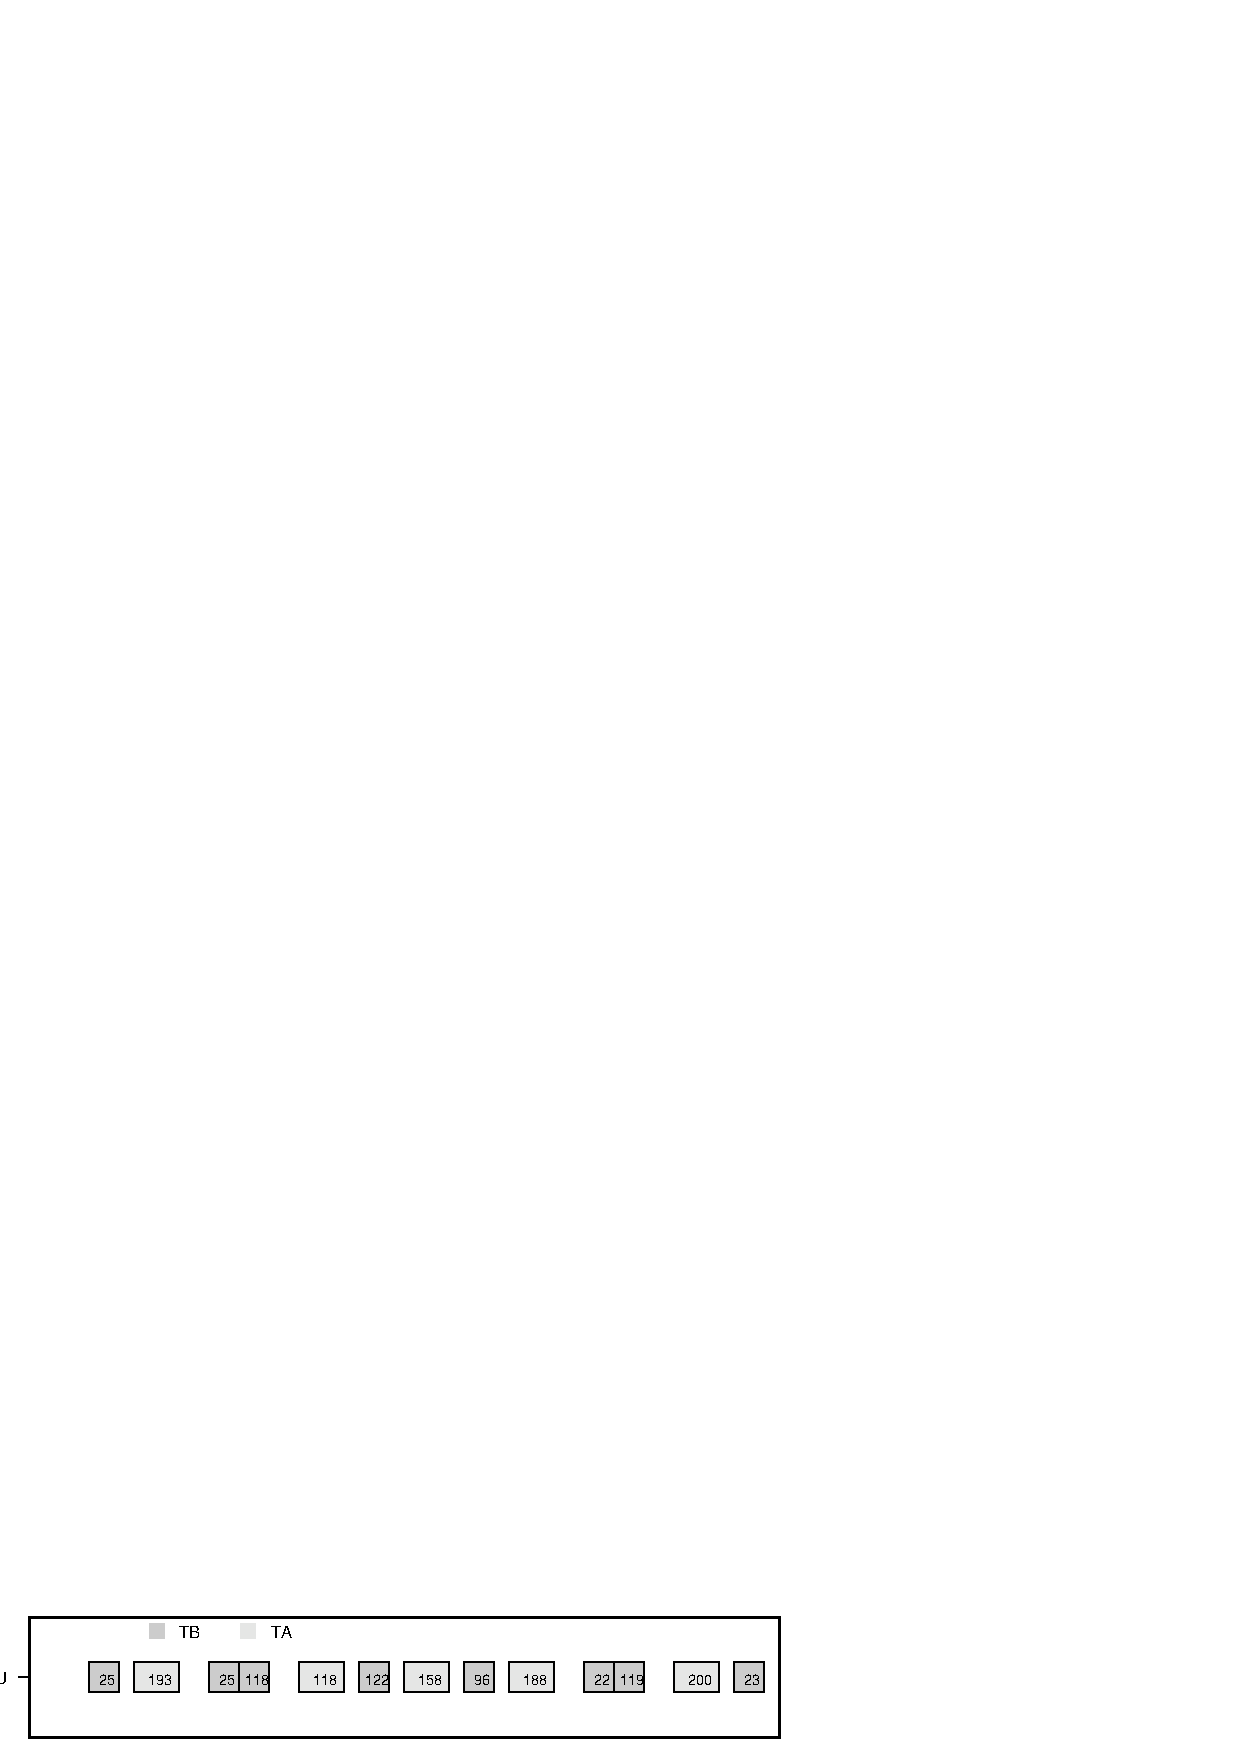
\includegraphics[scale=0.5]{TS_gantt.pdf}
\end{figure}
\begin{itemize}
\item Top: No terminal constraints; Bottom: Terminal constraints
\item Since we allow backorders, rolling horizon problem without
  terminal constraints is feasible
\item Terminal constraint: End at a periodic solution state (obtained
  for nominal demands)
\item \alert{Notice} larger batches with terminal constraints
\end{itemize}
\end{frame}

\begin{frame}{Integrating scheduling and inventory control}
\begin{figure}
\centering 
\scriptsize
\resizebox{0.75\textwidth}{!}{% GNUPLOT: LaTeX picture with Postscript
\begingroup
  \makeatletter
  \providecommand\color[2][]{%
    \GenericError{(gnuplot) \space\space\space\@spaces}{%
      Package color not loaded in conjunction with
      terminal option `colourtext'%
    }{See the gnuplot documentation for explanation.%
    }{Either use 'blacktext' in gnuplot or load the package
      color.sty in LaTeX.}%
    \renewcommand\color[2][]{}%
  }%
  \providecommand\includegraphics[2][]{%
    \GenericError{(gnuplot) \space\space\space\@spaces}{%
      Package graphicx or graphics not loaded%
    }{See the gnuplot documentation for explanation.%
    }{The gnuplot epslatex terminal needs graphicx.sty or graphics.sty.}%
    \renewcommand\includegraphics[2][]{}%
  }%
  \providecommand\rotatebox[2]{#2}%
  \@ifundefined{ifGPcolor}{%
    \newif\ifGPcolor
    \GPcolortrue
  }{}%
  \@ifundefined{ifGPblacktext}{%
    \newif\ifGPblacktext
    \GPblacktexttrue
  }{}%
  % define a \g@addto@macro without @ in the name:
  \let\gplgaddtomacro\g@addto@macro
  % define empty templates for all commands taking text:
  \gdef\gplbacktext{}%
  \gdef\gplfronttext{}%
  \makeatother
  \ifGPblacktext
    % no textcolor at all
    \def\colorrgb#1{}%
    \def\colorgray#1{}%
  \else
    % gray or color?
    \ifGPcolor
      \def\colorrgb#1{\color[rgb]{#1}}%
      \def\colorgray#1{\color[gray]{#1}}%
      \expandafter\def\csname LTw\endcsname{\color{white}}%
      \expandafter\def\csname LTb\endcsname{\color{black}}%
      \expandafter\def\csname LTa\endcsname{\color{black}}%
      \expandafter\def\csname LT0\endcsname{\color[rgb]{1,0,0}}%
      \expandafter\def\csname LT1\endcsname{\color[rgb]{0,1,0}}%
      \expandafter\def\csname LT2\endcsname{\color[rgb]{0,0,1}}%
      \expandafter\def\csname LT3\endcsname{\color[rgb]{1,0,1}}%
      \expandafter\def\csname LT4\endcsname{\color[rgb]{0,1,1}}%
      \expandafter\def\csname LT5\endcsname{\color[rgb]{1,1,0}}%
      \expandafter\def\csname LT6\endcsname{\color[rgb]{0,0,0}}%
      \expandafter\def\csname LT7\endcsname{\color[rgb]{1,0.3,0}}%
      \expandafter\def\csname LT8\endcsname{\color[rgb]{0.5,0.5,0.5}}%
    \else
      % gray
      \def\colorrgb#1{\color{black}}%
      \def\colorgray#1{\color[gray]{#1}}%
      \expandafter\def\csname LTw\endcsname{\color{white}}%
      \expandafter\def\csname LTb\endcsname{\color{black}}%
      \expandafter\def\csname LTa\endcsname{\color{black}}%
      \expandafter\def\csname LT0\endcsname{\color{black}}%
      \expandafter\def\csname LT1\endcsname{\color{black}}%
      \expandafter\def\csname LT2\endcsname{\color{black}}%
      \expandafter\def\csname LT3\endcsname{\color{black}}%
      \expandafter\def\csname LT4\endcsname{\color{black}}%
      \expandafter\def\csname LT5\endcsname{\color{black}}%
      \expandafter\def\csname LT6\endcsname{\color{black}}%
      \expandafter\def\csname LT7\endcsname{\color{black}}%
      \expandafter\def\csname LT8\endcsname{\color{black}}%
    \fi
  \fi
  \setlength{\unitlength}{0.0500bp}%
  \begin{picture}(7200.00,3024.00)%
    \gplgaddtomacro\gplbacktext{%
      \csname LTb\endcsname%
      \put(946,714){\makebox(0,0)[r]{\strut{} 0}}%
      \put(946,919){\makebox(0,0)[r]{\strut{} 10}}%
      \put(946,1123){\makebox(0,0)[r]{\strut{} 20}}%
      \put(946,1328){\makebox(0,0)[r]{\strut{} 30}}%
      \put(946,1532){\makebox(0,0)[r]{\strut{} 40}}%
      \put(946,1737){\makebox(0,0)[r]{\strut{} 50}}%
      \put(946,1941){\makebox(0,0)[r]{\strut{} 60}}%
      \put(946,2146){\makebox(0,0)[r]{\strut{} 70}}%
      \put(946,2350){\makebox(0,0)[r]{\strut{} 80}}%
      \put(946,2555){\makebox(0,0)[r]{\strut{} 90}}%
      \put(946,2759){\makebox(0,0)[r]{\strut{} 100}}%
      \put(1078,484){\makebox(0,0){\strut{} 0}}%
      \put(2223,484){\makebox(0,0){\strut{} 10}}%
      \put(3368,484){\makebox(0,0){\strut{} 20}}%
      \put(4513,484){\makebox(0,0){\strut{} 30}}%
      \put(5658,484){\makebox(0,0){\strut{} 40}}%
      \put(6803,484){\makebox(0,0){\strut{} 50}}%
      \put(176,1731){\rotatebox{-270}{\makebox(0,0){\strut{}Backorder -Retailer}}}%
      \put(3940,154){\makebox(0,0){\strut{}Time}}%
    }%
    \gplgaddtomacro\gplfronttext{%
      \csname LTb\endcsname%
      \put(5816,2586){\makebox(0,0)[r]{\strut{}Without terminal constraint}}%
      \csname LTb\endcsname%
      \put(5816,2366){\makebox(0,0)[r]{\strut{}With terminal constraint}}%
    }%
    \gplbacktext
    \put(0,0){\includegraphics{BOprofile}}%
    \gplfronttext
  \end{picture}%
\endgroup
}
\end{figure}
\begin{itemize}
\item Larger batches meant that \alert{more orders were met}
\item \alert{Inherent robustness}
\end{itemize}
\end{frame}

{\NoHeaderFooter
\begin{frame}{Outline-II}
\begin{itemize}
\item Distributed nature of supply chain decision making \\
 \centerline{\alert{ How to coordinate multiple decision makers?}}
\item Sharing information does not imply better
  solutions\footnote{minimize overall system cost}  

\item \alert{Distributed} MPC enables use of many interacting decision
  makers to improve overall system performance\footnotemark[\value{footnote}] 

\item Contributions:
 \begin{enumerate}
   \item {\color{blue}{Stability \& convergence guarantees extended to cover supply
     chain models}} 
   \item {\color{gray} {Robust cooperative MPC to design controllers
       that are robust to demand fluctuations}}
 \end{enumerate}
\end{itemize}
\end{frame}
}

\begin{frame}{2 node supply chain example}
  \begin{figure}
   \centering
   \resizebox{0.75\textwidth}{!}{\Large \begin{picture}(0,0)%
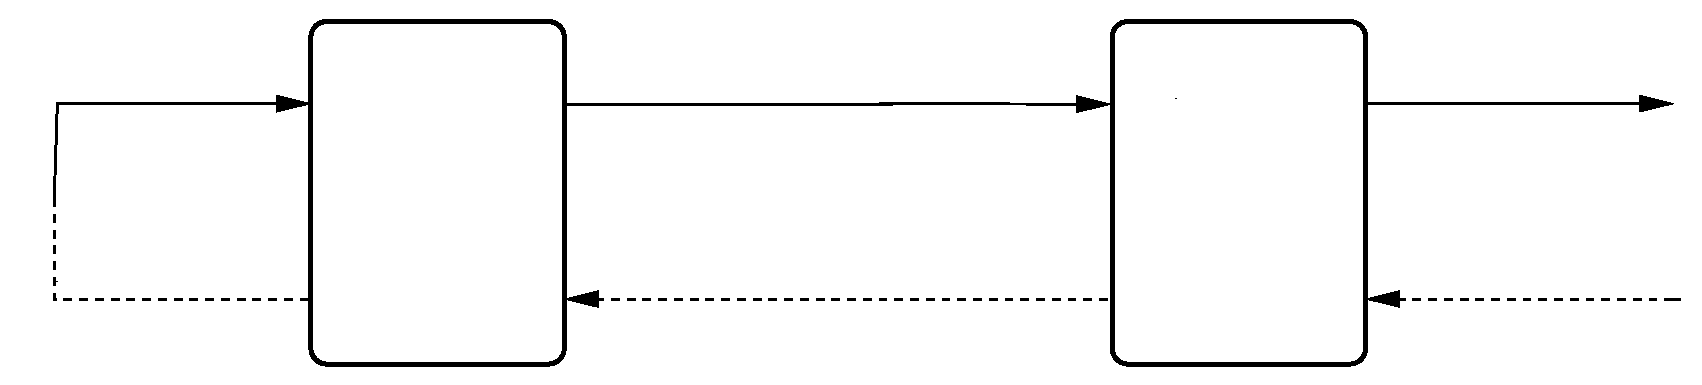
\includegraphics{sc/2node}%
\end{picture}%
\setlength{\unitlength}{4144sp}%
%
\begingroup\makeatletter\ifx\SetFigFont\undefined%
\gdef\SetFigFont#1#2#3#4#5{%
  \reset@font\fontsize{#1}{#2pt}%
  \fontfamily{#3}\fontseries{#4}\fontshape{#5}%
  \selectfont}%
\fi\endgroup%
\begin{picture}(10914,2274)(1114,-4123)
\put(1936,-3796){\makebox(0,0)[lb]{\smash{{\SetFigFont{12}{14.4}{\familydefault}{\mddefault}{\updefault}{\color[rgb]{0,0,0}$S_{2p}(k)$}%
}}}}
\put(11116,-3841){\makebox(0,0)[lb]{\smash{{\SetFigFont{12}{14.4}{\familydefault}{\mddefault}{\updefault}{\color[rgb]{0,0,0}$dem_{1c}(k)$}%
}}}}
\put(1576,-2266){\makebox(0,0)[lb]{\smash{{\SetFigFont{12}{14.4}{\familydefault}{\mddefault}{\updefault}{\color[rgb]{0,0,0}$S_{2p}(k-\tau_M)$}%
}}}}
\put(3106,-2986){\makebox(0,0)[lb]{\smash{{\SetFigFont{14}{16.8}{\familydefault}{\mddefault}{\updefault}{\color[rgb]{0,0,0}Manufacturer}%
}}}}
\put(8641,-2986){\makebox(0,0)[lb]{\smash{{\SetFigFont{14}{16.8}{\familydefault}{\mddefault}{\updefault}{\color[rgb]{0,0,0}Retailer}%
}}}}
\put(6166,-2491){\makebox(0,0)[lb]{\smash{{\SetFigFont{10}{12.0}{\familydefault}{\mddefault}{\updefault}{\color[rgb]{0,0,0}$\tau_T=2$}%
}}}}
\put(1171,-3031){\makebox(0,0)[lb]{\smash{{\SetFigFont{10}{12.0}{\familydefault}{\mddefault}{\updefault}{\color[rgb]{0,0,0}$\tau_M = 2$}%
}}}}
\put(8686,-3301){\makebox(0,0)[lb]{\smash{{\SetFigFont{12}{14.4}{\familydefault}{\mddefault}{\updefault}{\color[rgb]{0,0,0}Node $1$}%
}}}}
\put(9991,-2311){\makebox(0,0)[lb]{\smash{{\SetFigFont{12}{14.4}{\familydefault}{\mddefault}{\updefault}{\color[rgb]{0,0,0}$S_{1c}(k)$}%
}}}}
\put(7201,-3886){\makebox(0,0)[lb]{\smash{{\SetFigFont{12}{14.4}{\familydefault}{\mddefault}{\updefault}{\color[rgb]{0,0,0}$O_{12}(k)$}%
}}}}
\put(4816,-2716){\makebox(0,0)[lb]{\smash{{\SetFigFont{12}{14.4}{\familydefault}{\mddefault}{\updefault}{\color[rgb]{0,0,0}$S_{21}(k)$}%
}}}}
\put(3421,-3301){\makebox(0,0)[lb]{\smash{{\SetFigFont{12}{14.4}{\familydefault}{\mddefault}{\updefault}{\color[rgb]{0,0,0}Node $2$}%
}}}}
\end{picture}%
}
  \end{figure}
 \begin{itemize}
  \item Transportation delay: 1 time unit. Manufacturing delay: 2 time units.
  \item {\color{gray}{{Economic control objective}: Minimize operating cost
    \begin{multline*}\ell_E(x,u) = \text{Inventory holding cost}  \\+ \text{Production and Shipping cost} + \text{Lost order/sales cost} \end{multline*}}}
   \item {\alert{Distributed tracking control objective}: Cooperatively minimize tracking cost
      \[ \ell_T(x,u;z_p) = \norm{x-x_{\text{safety}}}_Q^2 + \norm{u-u_{\text{safety}}}_R^2\]}
  \item \alert{Nominal demand}: 8 units every time period. 
 \end{itemize}
\end{frame}

\begin{frame}{Supply chain policies}
\begin{itemize}
\item \alert{Retailer model:}
{\tiny{\begin{equation*}
\underbrace{\begin{bmatrix}\Inv_1\\\BO_1\end{bmatrix}_{k+1}}_{x_1(k+1)} =
\underbrace{\begin{bmatrix}1&\\ &
    1\end{bmatrix}}_{A_1}\underbrace{\begin{bmatrix}\Inv_1\\\BO_1\end{bmatrix}_k}_{x_1(k)}
+\underbrace{\begin{bmatrix}-1 & \alert{0} \\-1&
    \alert{0} \end{bmatrix}}_{B_{11}}\underbrace{\begin{bmatrix}S_{1c}\\O_{12}\end{bmatrix}_k}_{u_1(k)}
+\underbrace{\begin{bmatrix}-1 & 0 \\0&
    0 \end{bmatrix}}_{B_{21}^{(2)}}\underbrace{\begin{bmatrix}S_{21}\\S_{2m}\end{bmatrix}_{k-2}}_{u_2(k-2)}
+\underbrace{\begin{bmatrix} 0\\1\end{bmatrix}}_{B_d}\underbrace{\begin{bmatrix}\Dem_{1c}\end{bmatrix}_{k}}_{d(k)}
\end{equation*}
}}
\item \alert{Pull system}: Orders (Demands) initiate shipments  
 \item Individual node models do not contain enough information to
   predict how local orders affect future inventory.
   \newline
{\color{blue}{Each node needs to {\em{predict}} how the other nodes
    behave}}  
  \item \alert{Order-up-to policy (ord):} ``proportional controller''
   \begin{equation*}
      O_{12}(k) = \begin{cases} \Inv_t-\Inv_1(k) & \text{if $\Inv_1 \leq \Inv_t$} \\
             0 & \text{otherwise}  \end{cases}
   \end{equation*}
  \item \alert{Inventory position control (IP):} Define a new ``controlled output''
   \begin{equation*}
    \IP(k) = \Inv_1(k)-S_{1c}(k) + O_{12}(k)
   \end{equation*}
 \end{itemize}
 
\centerline{\color{blue}{Incomplete information + Model mismatch $\implies$ poor performance}}
\end{frame}

\begin{frame}{Noncooperative MPC}
\begin{figure}
 \centering
  \resizebox{0.7\textwidth}{!}{\input{sS_demand1}}
\end{figure}
\begin{itemize}
 \item Information shared among nodes. Each node knows the other
     nodes shipments and orders
   \item Nodes decide ordering based on a supply chain policy
   \item Each node minimizes its \alert{\it{local}} control objective
   \item \alert{Game theoretic result:} Solution converges to the Nash
     equilibrium
   \item Nash Equilibrium could \alert{destabilize} the plant
\end{itemize}
\end{frame}


\newsavebox{\Vcentral}
\savebox{\Vcentral}{\LARGE $V_1(\Redm{x_1},\Bluem{x_2},\Redm{\mathbf{u_1}},\Bluem{\mathbf{u_2}})+V_2(\Redm{x_1},\Bluem{x_2},\Redm{\mathbf{u_1}},\Bluem{\mathbf{u_2}})$}
\begin{frame}{Cooperative MPC: two players}
 \begin{columns}
  \begin{column}{0.5\textwidth}
   {\color{uwred}{Centralized MPC}}
   {\scriptsize
    \begin{gather*}
     \min_{\Redm{\mathbf{u_1}},\Bluem{\mathbf{u_2}}} 
     V_1(\Redm{x_1},\Bluem{x_2},\Redm{\mathbf{u_1}},\Bluem{\mathbf{u_2}})+V_2(\Redm{x_1},\Bluem{x_2},\Redm{\mathbf{u_1}},\Bluem{\mathbf{u_2}}) \\
     \text{s.t.~}\begin{bmatrix}\Redm{x_1}\\\Bluem{x_2}\end{bmatrix}^{+} = \begin{bmatrix}A_1 &
     \\ & A_2\end{bmatrix}\begin{bmatrix}\Redm{x_1}\\\Bluem{x_2}\end{bmatrix} +
     \begin{bmatrix}B_{11} & B_{12}
     \\B_{21} & B_{22}\end{bmatrix}\begin{bmatrix}\Redm{u_1}\\\Bluem{u_2}\end{bmatrix}\\
     \Redm{u_1} \in \mathbb{U}_1 \qquad \Bluem{u_2} \in \mathbb{U}_2\\
     x(N) = (x_1(N),x_2(N)) \in \mathbb{X}_f
    \end{gather*}
   }
  \end{column}
  \begin{column}{0.5\textwidth}
   \begin{center}
    \resizebox{0.5\textwidth}{!}{\multiinclude[format=tex,useinput]{suboptimal}}
   \end{center}
  \end{column}
 \end{columns}

 {\color{uwred}{Cooperative MPC}}
  \begin{itemize}
   \item Each subsystem solves for \textit{its local decision variables}
   \item<3-> Each iterate is \alert{feasible}
   \item<4-> Iterations converge to \alert{centralized optimal} solution$^*$
   \item<5-> Equivalent to \textit{Gauss-Jacobi} parallel optimization algorithm
   to solve the centralized problem
   \item<6-> Closed-loop stability and asymptotic convergence
     established using \alert{suboptimal MPC}
  \end{itemize}
\end{frame}
{\FooterCite{\citet{pannocchia:rawlings:wright:2011}}
\begin{frame}{Stability theory: Suboptimal MPC}
\begin{itemize} 
\item \alert{Cost function}: \qquad $\displaystyle V_N = \sum_{j=0}^{N-1}
  \underbrace{\ell(x(j), u(j))}_{\text{positive semi-definite stage cost}} + \alert{V_f(x(N))}$
\item \alert{Optimization}: \qquad $\displaystyle \min_{\bu} V_N (\bu,
  x(0)) $\\
subject to: \\
\centerline{$\bu = \{u(0), u(1), \ldots u(N-1)\}$}
\centerline{$x^+=Ax+Bu$ \qquad   $\alert{x(N) \in \mathbb{X}_f}$
  \qquad $\bu \in \mathbb{U}^N$} 
\item In Terminal region $\mathbb{X}_f$, $\exists$ terminal controller $\kappa_f(x)$
\item Consider \alert{feasible input sequence} $\bu=(u(0),u(1),\ldots,u(N-1))$ for state $x$.
\[ \bu \in \mathbb{U}^N \qquad x(N) \in \mathbb{X}_f\]
\item For successor state $x^+ = Ax + Bu^0(x)$, consider \alert{warm
  start}
\[ \tilde{\bu} = (u(1),u(2),\ldots,u(N-1),\kappa_f(x(N))\]
\end{itemize}
\end{frame}
}
{\FooterCite{\citet{pannocchia:rawlings:wright:2011}}
\begin{frame}{Stability theory: Suboptimal MPC}
\begin{itemize}
\item Warm start is feasible due to properties of $\mathbb{X}_f$
\item Warm start satisfies cost decrease due to properties of
  $\mathbb{X}_f $ \& $V_f(\cdot)$.
\[ V_N(x^+,\tilde{\bu}) - V_N(x,\bu) \leq -\ell(x,u(x))\]
\item Choose \alert{any} input $\bu^+$ such that
\[ V_N(x^+,\bu^+) \leq V_N(x^+,\tilde{\bu}) \]
\item We can show that {\color{blue}{$V_N(x,\bu)$ is a Lyapunov
    function.}}
\end{itemize} 



\end{frame}
}

\begin{frame}{Stability theory: Cooperative MPC}
\begin{itemize}
\item Warm start ensures that $V_N(x^+,\tilde{\bu}) - V_N(x,\bu) \leq -\ell(x,u(x))$
\item Jacobi iterations ensures that 
  \[ V_N(x^+, \bu^+) \leq V_N(x^+,\tilde{\bu}) \qquad \bu^+
  \text{~feasible}
\]
\item {\color{blue}{Cooperative MPC $\subset$ suboptimal MPC}}
 
\item \alert{Cooperative control $\rightarrow$ centralized control}
\begin{itemize}
  \item Jacobi iterations converge to centralized solution for
    \alert{uncoupled constraints}
  \item Coupled constraints in MPC:
    \begin{enumerate}
      \item State constraints
     \item Input constraints: 
     \item Terminal constraints
   \end{enumerate}
\end{itemize} 
\item Two techniques:
\begin{enumerate}
\item Decouple the terminal equality constraint $x(N) = x_S$
  \citep{stewart:venkat:rawlings:wright:pannocchia:2010} \\
  \centerline{{\color{blue}{Not applicable for supply chain systems}}}  
\item \alert{Relaxing the terminal region constraint}
\end{enumerate}
\end{itemize}
\end{frame}


{\FooterCite{\citet{subramanian:rawlings:maravelias:2012,pannocchia:rawlings:wright:2011,stewart:wright:rawlings:2011}}
\begin{frame}{Relaxation}
\begin{itemize}
 \item  Steer $x$ to an ellipsoidal terminal region using parameter
     $\Redm{a > 0}$ \newline
    \centerline{{$\displaystyle \mathbb{X}_f:= \set{x \mid  V_f(x) = x'Px \leq a \qquad a > 0}$}}
   
 \item Modify optimization problem using parameter $\Redm{\beta\geq 1}$:
   \[ \min_{\bu \in \mathbb{U}^N}{V_N^{\Redm{\beta}}(x,\bu) =
     \sum_{j=0}^{N-1}\ell(x(j),u(j)) + \Redm{\beta}V_f(x(N))}\]
      
 \item Modify Admissible region using parameter $\Redm{\bar{V} \geq a}$
  $\displaystyle \mathbb{Z}_N^{\Redm{\beta}} = \set{(x,\bu) \vert
    \exists \bu \in \mathbb{U}^N \text{s.t~} V_N^{\Redm{\beta}} \leq
    \bar{V}}$
  
\item Choose $\Redm{\beta}= \frac{\bar{V}} {a}$
 
\item Can show that for every $(x,\bu) \in \mathbb{Z}_N^{\beta}$,
  terminal region constraint is satisfied.  
\end{itemize}
\end{frame}
}

\begin{frame}{Results}
\begin{figure}
 \centering
  \resizebox{1\textwidth}{!}{\input{sS_demand}}
\end{figure}
\centerline{Significant improvement with just 1 iteration of
  cooperative control}
\end{frame}

{\NoHeaderFooter 
\begin{frame}{Outline-II}
\begin{itemize}
\item Distributed nature of supply chain decision making \\
 \centerline{\alert{ How to coordinate multiple decision makers?}}
\item Sharing information does not imply better
  solutions\footnote{minimize overall system cost}  

\item \alert{Distributed} MPC enables use of many interacting decision
  makers to improve overall system performance\footnotemark[\value{footnote}] 

\item Contributions:
 \begin{enumerate}
   \item {\color{gray}{Stability \& convergence guarantees extended to cover supply
     chain models}} 
   \item {\color{blue} {Robust cooperative MPC to design controllers
       that are robust to demand fluctuations}}
 \end{enumerate}
\end{itemize}
\end{frame}
}

% \begin{frame}{Robust cooperative control}
% \begin{itemize}
% \item Coupled constraints enforced implicitly
%  \begin{itemize}
%    \item Only $(x,\bu)$ pairs in $\mathbb{Z}_N^\beta = \set{(x,\bu) \vert
%     \exists \bu \in \mathbb{U}^N \text{s.t~} V_N^{\Redm{\beta}} \leq
%     \bar{V}}$ ensure that terminal region constraint is satisfied.
%   \item For state $x$ and input $\bu$, warm start $\tilde{\bu}$ is
%     \alert{constructed} such that $(x^+,\tilde{\bu}) \in
%     \mathbb{Z}_N^\beta$.
%  \end{itemize}
% \item For various reasons, the successor state need not be equal to
%   the predicted state
%    \begin{itemize}
%     \item Plant-model mismatch
%     \item Unmodeled disturbance
%     \item \alert{Not observing the nominal demand}
%   \end{itemize}
% \item Need control to be robust!
% \end{itemize}
% \end{frame}

% {\FooterCite{\citet{langson:chryssochoos:rakovic:mayne:2004}}
% \begin{frame}{Tube based MPC for robust control}
% \begin{itemize}
% \item \alert{Actual system}: $x^+ = Ax + Bu +{\color{blue}{d}}$  
% \item \alert{Nominal system}: $ z^+ = Az + Bv$  
% \item \alert{Error dynamics}: $ e^+ = (x-z)^+ = Ae + B(u-v) + d$  
% \item \alert{Basic idea}
%   \begin{itemize}
%     \item Obtain \alert{optimal input} for the nominal system $\mathbf{v}(z)$ using MPC  
%     \item \alert{Correct for disturbances} using the error signal  $ u = v + K(x-z)$ . 
%    \end{itemize}
% \item \alert{Controlled system:}
% \[ x^+ = Ax + Bv + BK(x-z) + d \qquad z^+ = Az + Bv \]
% \item \alert{Interpretation} 
% \newline
% {\color{blue} {The state $x$ lies in a bundle (tube) characterized by
%     $\mathbb{W}$, $K$ and the nominal control law $v = \kappa(z)$}}
% \end{itemize}
% \end{frame}
% }

% \begin{frame}{Tube based MPC}
% \begin{itemize}
%  \item $e^+ = (x-z)^+ = (A+BK)e + d$
%  \item Choose $K$ so that $A_K :=(A+BK)$ is stable
%  \item Can show that $ e \in S_K(\infty) := \sum_{i=0}^{\infty}A_K^{i}\mathbb{W}$
% \item Tighten the constraints so that 
% \[ z\in \mathbb{Z} \implies x \in \mathbb{X} \qquad v \in \mathbb{V} \implies u \in \mathbb{U}\]
% \item $\mathbb{Z},\mathbb{V}$ depend on $K$ and $\mathbb{W}$
% \item Design stable MPC for the nominal system
% \end{itemize}
% \centerline{\color{blue}{Asymptotically $z \rightarrow {0}$ and $ e \rightarrow S_K(\infty)$}}
% \end{frame}

% \begin{frame}{Tube based robust cooperative control}             
% \begin{itemize}
% \item Warm start is always feasible (by design) for the nominal system
% \item \alert{Design cooperative MPC for the nominal system}
% \item Each subsystem finds input as:
%  \[ u_1 = v_1 + K_1 e \qquad u_2 = v_2 + K_2 e \]
% \item Subsystems share:
%  \begin{itemize}
%  \item Centralized model and objective
%  \item  $K = \begin{bmatrix} K_1 & K_2 \end{bmatrix}$ such that
%   centralized $A+BK$ is stable
%  \item Centralized \alert{actual \& nominal} states at each time
%  \end{itemize}
% \end{itemize}
% \end{frame}

% \begin{frame}{Example}
% \begin{figure}
%   \centering
%   \resizebox{0.7\textwidth}{!}{\input{CL1}}
% \end{figure}
% \begin{itemize}
% \item Cooperative MPC for nominal demand
% \item Gain $K$ chosen such that all unmet demands from time $t-1$ is
%   met at time $t$
% \item Extra shipments if actual demand is less than nominal demand :
%   \alert{No state constraints}
% \end{itemize}
% \end{frame}

% \begin{frame}{Example}
% \begin{figure}
%   \centering
%   \resizebox{0.7\textwidth}{!}{% GNUPLOT: LaTeX picture with Postscript
\begingroup
  \makeatletter
  \providecommand\color[2][]{%
    \GenericError{(gnuplot) \space\space\space\@spaces}{%
      Package color not loaded in conjunction with
      terminal option `colourtext'%
    }{See the gnuplot documentation for explanation.%
    }{Either use 'blacktext' in gnuplot or load the package
      color.sty in LaTeX.}%
    \renewcommand\color[2][]{}%
  }%
  \providecommand\includegraphics[2][]{%
    \GenericError{(gnuplot) \space\space\space\@spaces}{%
      Package graphicx or graphics not loaded%
    }{See the gnuplot documentation for explanation.%
    }{The gnuplot epslatex terminal needs graphicx.sty or graphics.sty.}%
    \renewcommand\includegraphics[2][]{}%
  }%
  \providecommand\rotatebox[2]{#2}%
  \@ifundefined{ifGPcolor}{%
    \newif\ifGPcolor
    \GPcolortrue
  }{}%
  \@ifundefined{ifGPblacktext}{%
    \newif\ifGPblacktext
    \GPblacktexttrue
  }{}%
  % define a \g@addto@macro without @ in the name:
  \let\gplgaddtomacro\g@addto@macro
  % define empty templates for all commands taking text:
  \gdef\gplbacktext{}%
  \gdef\gplfronttext{}%
  \makeatother
  \ifGPblacktext
    % no textcolor at all
    \def\colorrgb#1{}%
    \def\colorgray#1{}%
  \else
    % gray or color?
    \ifGPcolor
      \def\colorrgb#1{\color[rgb]{#1}}%
      \def\colorgray#1{\color[gray]{#1}}%
      \expandafter\def\csname LTw\endcsname{\color{white}}%
      \expandafter\def\csname LTb\endcsname{\color{black}}%
      \expandafter\def\csname LTa\endcsname{\color{black}}%
      \expandafter\def\csname LT0\endcsname{\color[rgb]{1,0,0}}%
      \expandafter\def\csname LT1\endcsname{\color[rgb]{0,1,0}}%
      \expandafter\def\csname LT2\endcsname{\color[rgb]{0,0,1}}%
      \expandafter\def\csname LT3\endcsname{\color[rgb]{1,0,1}}%
      \expandafter\def\csname LT4\endcsname{\color[rgb]{0,1,1}}%
      \expandafter\def\csname LT5\endcsname{\color[rgb]{1,1,0}}%
      \expandafter\def\csname LT6\endcsname{\color[rgb]{0,0,0}}%
      \expandafter\def\csname LT7\endcsname{\color[rgb]{1,0.3,0}}%
      \expandafter\def\csname LT8\endcsname{\color[rgb]{0.5,0.5,0.5}}%
    \else
      % gray
      \def\colorrgb#1{\color{black}}%
      \def\colorgray#1{\color[gray]{#1}}%
      \expandafter\def\csname LTw\endcsname{\color{white}}%
      \expandafter\def\csname LTb\endcsname{\color{black}}%
      \expandafter\def\csname LTa\endcsname{\color{black}}%
      \expandafter\def\csname LT0\endcsname{\color{black}}%
      \expandafter\def\csname LT1\endcsname{\color{black}}%
      \expandafter\def\csname LT2\endcsname{\color{black}}%
      \expandafter\def\csname LT3\endcsname{\color{black}}%
      \expandafter\def\csname LT4\endcsname{\color{black}}%
      \expandafter\def\csname LT5\endcsname{\color{black}}%
      \expandafter\def\csname LT6\endcsname{\color{black}}%
      \expandafter\def\csname LT7\endcsname{\color{black}}%
      \expandafter\def\csname LT8\endcsname{\color{black}}%
    \fi
  \fi
  \setlength{\unitlength}{0.0500bp}%
  \begin{picture}(7200.00,3024.00)%
    \gplgaddtomacro\gplbacktext{%
      \csname LTb\endcsname%
      \put(814,704){\makebox(0,0)[r]{\strut{} 10}}%
      \put(814,1732){\makebox(0,0)[r]{\strut{} 20}}%
      \put(814,2759){\makebox(0,0)[r]{\strut{} 30}}%
      \put(946,484){\makebox(0,0){\strut{} 0}}%
      \put(1433,484){\makebox(0,0){\strut{} 10}}%
      \put(1921,484){\makebox(0,0){\strut{} 20}}%
      \put(2408,484){\makebox(0,0){\strut{} 30}}%
      \put(2896,484){\makebox(0,0){\strut{} 40}}%
      \put(3383,484){\makebox(0,0){\strut{} 50}}%
      \put(176,1731){\rotatebox{-270}{\makebox(0,0){\strut{}Level in Tank-1}}}%
      \put(2164,154){\makebox(0,0){\strut{}Time}}%
      \put(1921,1218){\makebox(0,0)[l]{\strut{}$S_K(\infty)$ bound}}%
    }%
    \gplgaddtomacro\gplfronttext{%
      \csname LTb\endcsname%
      \put(2396,2586){\makebox(0,0)[r]{\strut{}Actual}}%
      \csname LTb\endcsname%
      \put(2396,2366){\makebox(0,0)[r]{\strut{}Nominal}}%
    }%
    \gplgaddtomacro\gplbacktext{%
      \csname LTb\endcsname%
      \put(4109,484){\makebox(0,0){\strut{} 0}}%
      \put(4517,484){\makebox(0,0){\strut{} 2}}%
      \put(4925,484){\makebox(0,0){\strut{} 4}}%
      \put(5334,484){\makebox(0,0){\strut{} 6}}%
      \put(5742,484){\makebox(0,0){\strut{} 8}}%
      \put(6150,484){\makebox(0,0){\strut{} 10}}%
      \put(6282,704){\makebox(0,0)[l]{\strut{} 0}}%
      \put(6282,1115){\makebox(0,0)[l]{\strut{} 100}}%
      \put(6282,1526){\makebox(0,0)[l]{\strut{} 200}}%
      \put(6282,1937){\makebox(0,0)[l]{\strut{} 300}}%
      \put(6282,2348){\makebox(0,0)[l]{\strut{} 400}}%
      \put(6282,2759){\makebox(0,0)[l]{\strut{} 500}}%
      \put(7051,1731){\rotatebox{-270}{\makebox(0,0){\strut{}Cost}}}%
      \put(5129,154){\makebox(0,0){\strut{}Time}}%
    }%
    \gplgaddtomacro\gplfronttext{%
      \csname LTb\endcsname%
      \put(5163,2586){\makebox(0,0)[r]{\strut{}$V_N^\beta(x,\tilde{\mathbf{v}})$}}%
      \csname LTb\endcsname%
      \put(5163,2366){\makebox(0,0)[r]{\strut{}$V_N^\beta(z,\tilde{\mathbf{v}})$}}%
      \csname LTb\endcsname%
      \put(5163,2146){\makebox(0,0)[r]{\strut{}$\bar{V}$}}%
    }%
    \gplbacktext
    \put(0,0){\includegraphics{mpc/CL2}}%
    \gplfronttext
  \end{picture}%
\endgroup
}
%  \end{figure}
% \begin{itemize}
% \item The nominal MPC does not use ``feedback'' from the actual states
% \item \alert{Proposal:}\footnote{\citet{rawlings:mayne:2009}} To ``reset'' the nominal state to the actual
%   state if 
% \begin{enumerate}
% \item Cost-drop is guaranteed
% \item Warm start is feasible  
% \item Slow time scale restart (no convergence guarantees) 
% \end{enumerate}
% \end{itemize}
% \end{frame}

\begin{frame}{Conclusions}
\alert{Confirm previous observations:}
\begin{itemize}
\item Centralized optimization reduces bullwhip effect
\item Information sharing  can improve performance
\end{itemize} 
\alert{New results:}
\begin{itemize}
\item Design procedures for 
 \begin{itemize}
   \item Economic MPC for supply chain optimization
   \item Multiobjective MPC 
   \item Iterative scheduling
 \end{itemize}
\item Robust cooperative MPC algorithms
  \begin{itemize}
    \item Compatible with distributed nature of inventory control
    \item Efficient operation (if models and objective function can be
      shared)
   \end{itemize}
\end{itemize}
\end{frame}

\begin{frame}{Future work}
\begin{itemize}

\item Hybrid control theory

\item Impact of forecast

\item Terminal conditions 
 \begin{itemize}
   \item Robust vs Nominal
   \item For the scheduling problem
\end{itemize}
\item Cooperative game theory
\item Implementation
\end{itemize}


\end{frame}


{\NoHeaderFooter
 \begin{frame}[allowframebreaks]{References}
  \addtocounter{framenumber}{-2}
  \scriptsize
  \bibliographystyle{abbrvnat}
  \bibliography{abbreviations,articles,proceedings,books,unpub}%,resgrppub}
 \end{frame} 
}
\end{document}   
